\documentclass[12pt,letterpaper]{article}

\usepackage[T1]{fontenc}
\usepackage{tgtermes}
\usepackage[top=1in,bottom=1in,left=1.25in,right=1.25in]{geometry}
\usepackage{graphicx}
\usepackage{amsmath}
\usepackage{booktabs}
\usepackage{longtable}
\usepackage{array}
\usepackage{tabularx}
\usepackage{abstract}
\usepackage{caption}
\usepackage{microtype}
\usepackage{xurl}
\usepackage{setspace}
\usepackage{titlesec}
\usepackage{placeins}
\usepackage{float}
\usepackage[hidelinks]{hyperref}

\graphicspath{{../../figures/}}

\onehalfspacing
\setlength{\parindent}{1.5em}
\setlength{\parskip}{0pt}
\setlength{\emergencystretch}{3em}
\setlength{\textfloatsep}{14pt plus 3pt minus 4pt}
\setlength{\floatsep}{12pt plus 3pt minus 3pt}
\setlength{\intextsep}{12pt plus 3pt minus 3pt}
\renewcommand{\topfraction}{0.92}
\renewcommand{\bottomfraction}{0.85}
\renewcommand{\textfraction}{0.06}
\renewcommand{\floatpagefraction}{0.78}
\setcounter{topnumber}{2}
\setcounter{bottomnumber}{2}
\setcounter{totalnumber}{3}
\setlength{\absleftindent}{1.2em}
\setlength{\absrightindent}{1.2em}
\setlength{\absparsep}{0.5em}
\captionsetup{font=small,labelfont=bf,justification=raggedright,
  singlelinecheck=false,skip=7pt}
\captionsetup[longtable]{justification=centering,singlelinecheck=false}
\makeatletter
\setlength{\@fptop}{0pt}
\setlength{\@fpbot}{0pt plus 1fil}
\makeatother
\titleformat{\subsubsection}
  {\normalfont\normalsize\bfseries}{\thesubsubsection}{1em}{}
\titlespacing*{\section}{0pt}{1.35\baselineskip}{0.5\baselineskip}
\titlespacing*{\subsection}{0pt}{1.05\baselineskip}{0.4\baselineskip}
\titlespacing*{\subsubsection}{0pt}{0.85\baselineskip}{0.3\baselineskip}

\newcolumntype{L}[1]{>{\raggedright\arraybackslash}p{#1}}
\newcolumntype{R}[1]{>{\raggedleft\arraybackslash}p{#1}}
\newcolumntype{Y}{>{\raggedright\arraybackslash}X}
\newcolumntype{C}{>{\centering\arraybackslash}X}

\begin{document}
\pagenumbering{gobble}

\begin{titlepage}
\thispagestyle{empty}
\begin{center}
\vspace*{1.2cm}
{\Large Ritsumeikan Asia Pacific University\par}
\vspace{0.35cm}
{\large College of Sustainability and Tourism\par}
\vspace{1.1cm}
{\Large\bfseries Graduation Thesis\par}

\vfill

{\LARGE\bfseries Three Margins of Electricity Recovery\par}
\vspace{0.45cm}
{\Large Coverage, Reported Entry, and Generator Sizing in Japan's\par}
\vspace{0.15cm}
{\Large Municipal Incinerator Fleet, FY2005--FY2024\par}

\vfill

{\large Pann Phetra\par}
\vspace{0.4cm}
{\large Student ID: 13223029\par}
\vspace{0.4cm}
{\large Supervisor: Prof. Han Ji\par}

\vfill

{\large 19 July 2026\par}
\end{center}
\end{titlepage}

\clearpage
\pagenumbering{roman}

\begin{abstract}
Facility counts can misdiagnose electricity recovery when they collapse fleet
coverage, entry, and engineering performance into one statistic. This thesis
deterministically links 23,593 Japanese municipal-incinerator records from
fiscal year (FY) 2005 to FY2024 into 1,690 stable administrative lineages and
1,767 reported asset episodes. In FY2024, 41.1\%
of all records reported installed electrical capacity, but positive-output
facilities handled 80.1\% of recorded waste throughput. Facilities reporting
installed capacity represented 70.5\% of processing design capacity. The
all-record installed-capacity share rose by 19.5 percentage points from FY2005,
whereas the rise was 2.2 points among 732 lineages observed at both endpoints.
This contrast is consistent with a substantial contribution from changing
fleet composition. First reported capacity entry was rare: the primary
discrete-time model contained 35 events. At support-rich capacities of 24, 60,
and 120 tonnes per day, standardized annual risks were 0.68, 1.37, and 3.29
entries per 1,000 facility-years. A five-parameter Firth model gave a
300-versus-100 tonnes-per-day odds ratio of 6.72 (1,999-lineage-bootstrap 95\%
confidence interval: 4.31--12.46), although 300 tonnes per day was a thinly
supported tail value. The positive scale association survived continuity,
functional-form, reporting-state, leave-one-prefecture influence, and
event-influence checks. Among 6,511 engineering-valid generator-years from 493 lineages,
adjusted installed capacity was 79.1\%, 58.6\%, and 23.5\% lower in pre-1990,
1990s, and 2000s start-year cohorts than in the 2010-or-later cohort.
Administrative annual capacity-factor proxies were not uniformly lower in
older cohorts. Under common controls,
installed sizing was the largest absolute point-estimate accounting component
of each older cohort's log gross-generation-intensity gap. The exact component
sum is an identity, not independent causal evidence. The contribution is a
three-margin national diagnosis; it does not identify physical projects,
recoverable potential, or causal effects. Independent clerical review of the
highest-risk lineage links remains an outstanding validation step.
\end{abstract}

\vspace{0.15em}
\noindent\textbf{Keywords:} municipal solid waste; incineration; waste-to-energy;
Japan; generator sizing; capacity factor

\clearpage
\tableofcontents
\clearpage
\listoffigures
\addcontentsline{toc}{section}{List of Figures}
\vspace{1.5em}
\listoftables
\addcontentsline{toc}{section}{List of Tables}
\clearpage
\pagenumbering{arabic}

\section{Introduction}

Japan's municipal waste system relies extensively on incineration for volume
reduction and hygienic treatment. Electricity recovery can use part of the heat
released during combustion, but it does not by itself make incineration
preferable to prevention, reuse, or recycling. Its value depends on plant
design, waste properties, energy use, and the wider waste and electricity
systems (Astrup et al., 2009, 2015; Brunner \& Rechberger, 2015; European
Commission, 2017). Japan-specific work likewise extends beyond a binary label
of whether a plant generates electricity (Uno, 2015; Tabata \& Tsai, 2016;
Yamada et al., 2023).

The Ministry's FY2024 national summary reports 415 electricity-generating
facilities among 991 incineration facilities, or 41.9\% (Ministry of the
Environment Japan, 2026). That published context is distinct from this thesis's
analytical measure: 417 of 1,014 retained FY2024 facility records report
positive installed electrical capacity, or 41.1\%. The numerator definition and
record denominator differ, so the official ratio is not substituted into the
analytical calculations.

The most visible national statistic is often a facility count. Yet a small
intermittent facility and a large continuous facility each contribute one unit,
despite handling different waste volumes. A count describes how widely
equipment appears across records, not how much waste passes through generating
facilities or where processing capacity is located. Those are distinct coverage
questions.

A second problem arises in facility histories. First reporting of installed
capacity is uncommon and can occur within an administratively continuous
facility, with a reported asset reset, or in a forward-dated record. These cases
do not have one verified physical meaning. The workbooks also lack a reliable
identifier over the full period: codes are absent in FY2010--FY2012 and fully
change between FY2019 and FY2020. Treating them as persistent keys would break
histories and create false events.

A third problem concerns gross electricity divided by throughput. This gross
megawatt-hours-per-tonne (MWh/t) ratio combines generator size relative to
processing capacity, annual use of
installed electrical capacity, and waste loading. Treating it as an independent
operating measure can make a design-cohort difference look operational.

This thesis addresses the three problems in one national facility-level study.
It reconstructs stable administrative lineages before creating lags, separates
facility participation from waste-volume and design-capacity coverage, uses a
bias-reduced event-history model for sparse first-entry events, and decomposes
gross generation intensity into observable engineering components. The aim is
descriptive and diagnostic. The study does not estimate the effect of a
specific equipment project, infer a physical closure from administrative
absence, or calculate net electricity export, useful heat, lifecycle emissions,
or recoverable technical potential.

\subsection{Research questions}

The three research questions (RQs) are:

\begin{quote}
\textbf{RQ1: Coverage and fleet composition.} How did the share of facility
records reporting installed electrical-generation capacity evolve from FY2005
to FY2024; how does that count-based measure compare with the shares of recorded
waste throughput and processing design capacity covered by generating
facilities; and how much of the endpoint change remains among administrative
lineages observed in both years?
\end{quote}

\begin{quote}
\textbf{RQ2: First reported installed-capacity entry.} Among stable
administrative lineages first observed without installed electrical-generation
capacity, which prior-year age and waste-processing-scale profiles are
associated with first reporting positive capacity, and does the evidence change
after the risk set is restricted to lineages with positive prior-year waste
throughput?
\end{quote}

\begin{quote}
\textbf{RQ3: Installed design and annual use.} Among engineering-valid
operating-generator years, how do raw installed electrical capacity and annual
electrical capacity factor differ across reported facility start-year cohorts
after observed controls? Under a common control design, what are the relative
accounting components of cohort differences in gross MWh/t?
\end{quote}

The sequence matters. RQ1 establishes the denominator problem at fleet level.
RQ2 then asks which observed non-generating lineages enter the installed-capacity
state. RQ3 begins only after positive throughput and gross output are observed,
and asks what produces differences within the generating segment. Figure~\ref{fig:coverage}
shows the annual count, throughput, and design-capacity coverage measures that
anchor this sequence.

\noindent\begin{minipage}{\textwidth}
\medskip
\noindent\textbf{Reader map for the three research questions}

\begingroup
\small
\setlength{\tabcolsep}{4pt}
\renewcommand{\arraystretch}{1.12}
\begin{center}
\begin{tabularx}{\textwidth}{L{0.06\textwidth} L{0.20\textwidth} Y Y}
\toprule
RQ & Analysis population & Evidence approach & Interpretation boundary \\
\midrule
RQ1 & Full retained annual facility panel & Compare facility participation,
throughput coverage, design-capacity coverage, and endpoint-common change. &
Does not measure conversion efficiency, environmental optimality, or causal
retrofit. \\
RQ2 & Administrative lineages at risk of first reported installed-capacity
entry & Use a sparse-event Firth model to profile entry by prior-year age and
processing scale. & Does not identify a physical project date or the causal
effect of changing age or scale. \\
RQ3 & Engineering-valid operating-generator years & Model raw installed kW and
annual capacity factor, then reconcile the components of gross MWh/t. & Does
not measure net export, thermodynamic or lifecycle efficiency, or causal
mediation. \\
\bottomrule
\end{tabularx}
\end{center}
\endgroup
\end{minipage}

\begin{figure}[!htbp]
\centering
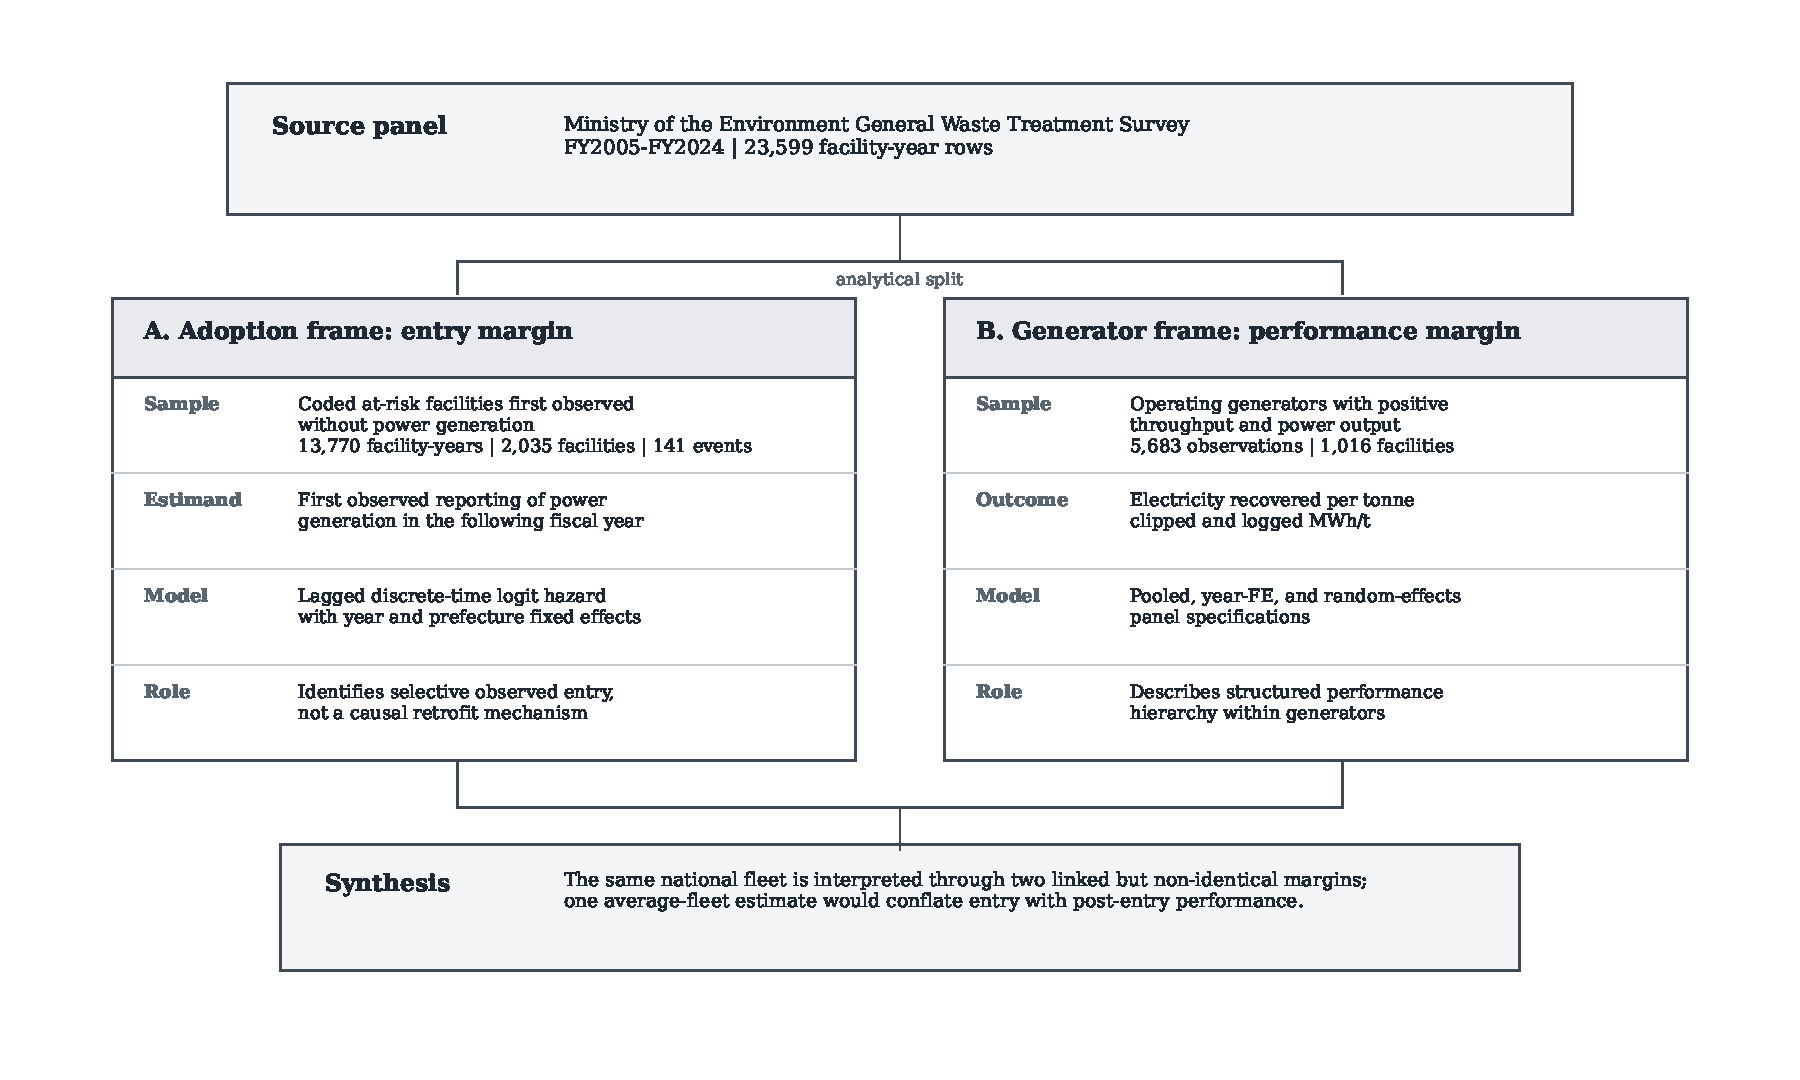
\includegraphics[width=0.86\textwidth,height=0.72\textheight,
  keepaspectratio]{figure1_two_part_framework.pdf}
\caption[Annual electricity-recovery coverage by denominator,
FY2005--FY2024]{Annual electricity-recovery coverage among retained Japanese
municipal-incinerator records, FY2005--FY2024. ``Facilities'' is the share of
records reporting positive installed electrical capacity; ``Throughput'' is
the share of annual waste processed at records reporting positive electricity
output; and ``Capacity'' is the share of total waste-processing design capacity
at records reporting positive installed electrical capacity. These three
denominators answer different questions and are not interchangeable.}
\label{fig:coverage}
\end{figure}

\subsection{Thesis objectives and significance}

The thesis has four linked objectives. First, it establishes a reproducible
longitudinal facility record before calculating transitions. This is necessary
because the official identifiers do not provide an uninterrupted key over the
study period. Second, it compares three fleet-coverage denominators rather than
allowing the facility count to stand for the whole system. Third, it estimates
first reported installed-capacity entry only within an explicit population at
risk and uses a sparse-event estimator suited to the small number of observed
entries. Fourth, it decomposes gross generation per tonne into generator design
intensity, electrical capacity factor, and waste-processing utilization. The
objectives therefore progress from data identity, to fleet description, to
transition, and finally to conditional engineering structure.

The academic significance lies primarily in this integrated measurement
architecture. Existing studies offer important analyses of system outcomes,
facility performance, and Japanese waste-to-energy policy, but those questions
do not share one denominator or one comparison population. Treating them as if
they did can turn a descriptive fleet share into a performance statement, or a
conditional generator comparison into an explanation of adoption. This thesis
shows how the three questions can be studied together without collapsing their
estimands. It also demonstrates why identity reconstruction is part of the
research design rather than a preliminary clerical step: transition estimates
depend on which annual records are considered continuous.

The practical significance is diagnostic rather than prescriptive. National
and municipal decision-makers need to know whether low participation by count
also means low coverage of waste activity, whether observed entry is broadly
distributed or concentrated among particular facility profiles, and whether a
gross-output difference reflects generator size or annual use. The results can
identify where additional engineering, financial, or project-history evidence
is most valuable. They cannot by themselves select a retrofit, replacement, or
closure project.

The social significance follows from keeping electricity recovery within the
waste hierarchy. Recovering electricity can reduce wasted combustion heat, but
it does not make waste prevention, reuse, and recycling unnecessary. Clear
measurement helps prevent a high throughput-coverage statistic from being
presented as proof of environmental optimality. It also avoids treating every
non-generating facility as an equally feasible opportunity when local waste
supply, costs, grid access, heat demand, and alternative treatment arrangements
remain unobserved.

\section{Literature Review}

\subsection{Waste-to-energy within the waste hierarchy}

Waste-to-energy (WtE) is not a single environmental outcome. It is a family of
thermal-treatment arrangements that can provide waste-disposal service, recover
electricity or useful heat, and produce emissions and residual materials at the
same time. Reviews therefore evaluate incineration within material-flow,
life-cycle, energy-system, and waste-hierarchy boundaries rather than by
electricity output alone (Astrup et al., 2009, 2015; Brunner \& Rechberger, 2015;
Lombardi et al., 2015; M\"{u}nster \& Meibom, 2010). The environmental value
assigned to recovered energy can change with waste composition, the energy
displaced, plant configuration, treatment alternatives, and the boundary chosen
for analysis.

This wider framing is especially important for a study of an incineration-heavy
system. Comparative policy research places prevention, reuse, and material
recycling ahead of disposal, while recognizing energy recovery as one possible
function of residual-waste treatment (European Commission, 2017; Sakai et al.,
2011). Increasing electricity recovery is therefore not equivalent to improving
the whole waste system. More generation could reflect better use of unavoidable
combustion heat, but it could also coexist with high residual-waste throughput.
The appropriate interpretation depends on which question is being asked.

This thesis deliberately conditions on the observed Japanese incineration fleet.
It asks how electricity recovery is distributed within that fleet, not whether
incineration should replace prevention or recycling. It also does not estimate
life-cycle greenhouse-gas savings, avoided generation, pollutant exposure, ash
management, heat use, or social welfare. Keeping these outcomes outside the
estimand prevents the gross electricity measures reported below from becoming
an unsupported claim of overall sustainability.

\subsection{Japan's municipal transition and operating context}

Japan's municipal solid-waste system combines national policy with local
implementation. Municipal instruments can alter the quantity and composition of
residual waste before it reaches an incinerator. For example, Japanese
unit-charging programmes have been studied as waste-reduction and recycling
measures, with effects depending on programme design and complementary
collection arrangements (Sakai et al., 2008). This means that annual incinerator
throughput is not simply an engineering input: it is partly the downstream result
of local waste-management choices that are not fully observed in the facility
workbooks.

Within the treatment stage, prior Japan-focused research examines several
different margins. Uno (2015) describes technical developments associated with
higher-efficiency power generation. Tabata and Tsai (2016) examine heat supply
and the local constraints on using recovered heat. Sun et al. (2018) show through
a Tokyo case that energy recovery can be considered within an integrated urban
waste-management network rather than at one plant in isolation. Sasao (2018)
uses repeated facility observations to study how municipal solid-waste policy
relates to heat and electricity output. Shino (2019) examines generation
performance relative to waste input, while Yamada et al. (2023) place the sector
within longer-run Japanese decarbonization scenarios.

The institutional setting also changed during the observation window. The
Ministry maintains a high-efficiency waste-power facility development manual
that links facility-support requirements to generation performance and plant
planning (Ministry of the Environment Japan, n.d.). The Great East Japan
Earthquake and Fukushima Daiichi accident in March 2011 then changed the
national energy-policy context. Japan's feed-in tariff (FIT) system began in
July 2012, and waste-derived biomass electricity was among the eligible
renewable categories (Agency for Natural Resources and Energy, 2017; Sasao,
2018). In FY2014, the Ministry also offered capital support for high-efficiency
waste-heat recovery and waste-derived biomass generation (Ministry of the
Environment Japan, 2014).

These milestones make calendar time substantively relevant, but do not create a
causal design here. The workbooks do not identify subsidy receipt, FIT
accreditation, electricity contracts, or investment motives. The entry model
therefore includes a smooth calendar term; it does not treat FY2011 or FY2012 as
an exogenous breakpoint or estimate a Fukushima or FIT effect.

Scale is important in this literature, but it is not a complete decision rule.
Large, continuously operated plants can support steam conditions and generating
equipment that are difficult to reproduce at small sites. Yet a heat-balance case
study by Yoshida et al. (2018) identifies technically possible recovery options
for a small Japanese facility and separately examines their costs and benefits.
The relevant question is therefore not simply whether a small plant lacks a
generator. Feasibility can also depend on waste supply, technology, capital and
operating costs, grid connection, heat demand, and regional coordination.

The national administrative panel used here does not consistently observe those
project-level factors. It can show which reported facility profiles are
associated with witnessed entry, but it cannot identify why a municipality made
a particular investment. This boundary is consequential: an association between
size and entry is evidence about observed selection in the fleet, not proof that
size alone caused adoption or that every large non-generator should be
retrofitted.

\subsection{Measuring coverage, performance, and efficiency}

The literature also shows why the word \emph{efficiency} requires qualification.
Thermal-treatment reviews compare technologies using electrical, thermal, or
combined energy performance and sometimes life-cycle measures (Astrup et al.,
2015; Lombardi et al., 2015). The European Union's R1 energy-recovery formula
uses a defined accounting boundary (Grosso et al., 2010).
Facility benchmarking studies may instead estimate technical or revenue
efficiency relative to observed peers (Chen et al., 2012; Yeh, 2020). These are
not interchangeable quantities.

The Ministry workbooks report installed electrical capacity, annual gross
electricity generation, waste-processing design capacity, and annual throughput.
They do not provide a complete and consistent series for net export, internal
electricity use, useful heat delivery, lower heating value, steam conditions,
operating cost, or emissions. Gross megawatt-hours per tonne (MWh/t) is therefore
observable, but it is not a direct thermal-conversion efficiency. Shino (2019)
similarly treats generation relative to waste input as informative while noting
that a thermal interpretation requires calorific-value information.

Measurement also changes the apparent reach of energy recovery. A facility-count
share weights a small and a large plant equally. A throughput share weights each
plant by the tonnes it actually processes. A design-capacity share weights its
nominal daily waste-processing capacity. None is inherently the correct
denominator for every purpose. Used together, however, they reveal whether
generation is diffuse across facilities or concentrated where most waste is
processed and capacity is installed.

The present design consequently separates three estimands. Fleet coverage is an
annual ratio whose denominator is facilities, tonnes, or waste-processing design
capacity. Entry is a discrete-time conditional probability among lineages
observed at risk. Generator-component estimates are conditional associations
among positive-throughput, positive-output generator-years that pass stated
engineering checks. A coefficient from the generator frame cannot explain why a
non-generator enters, and a facility participation rate cannot describe the
share of waste processed with electricity output.

This separation permits a low count share and high throughput share to be true
simultaneously. It also permits newer cohorts to report higher gross MWh/t
because of larger generators even when older generators do not have lower annual
capacity factors. Section~3 states the exact identity used to distinguish those
components.

\subsection{Infrastructure heterogeneity, transition, and persistence}

Incinerators are long-lived infrastructure embedded in municipal organisations,
regulation, collection systems, energy networks, and local service obligations.
Socio-technical research distinguishes a technology from the wider system of
actors, rules, users, and material arrangements that supports it (Geels, 2004).
Carbon lock-in research likewise explains how long-lived capital and
institutional interdependence can make infrastructure pathways persistent
(Seto et al., 2016; Unruh, 2000). These perspectives make age, cohort, and
continuity relevant, but they do not establish that every old incinerator is
technically or politically locked in.

This thesis uses that literature as a conceptual warning rather than a tested
causal theory. The workbooks do not observe investment deliberations, sunk
costs, procurement contracts, or political opposition. They also do not show
whether first reported generation was installed through an in-place retrofit, a
furnace replacement, a wider site redevelopment, or correction of a previous
record. Accordingly, the longitudinal unit is called a stable administrative
lineage, and large configuration changes create separate asset episodes. A
first-entry event means the first witnessed transition from no reported
generation to reported generation under a stated continuity rule; it is not
automatically labelled a retrofit.

This distinction explains why identity reconstruction is substantive. If a
national recoding is mistaken for facility replacement, apparent entry and exit
events will be manufactured by the database. If all records sharing a site name
are forced into one permanent asset, genuine replacement may be hidden. The
lineage and episode sensitivity analyses translate the general infrastructure
literature into a testable question: how much do transition inferences depend on
the continuity definition?

\subsection{Methodological comparators and adaptation}

Recent studies supply research logic, not a ready-made model. Cui et al.
(2026) foreground facility hierarchy, Liu et al. (2025) emphasize effectiveness
over expansion, and Han et al. (2025) place recovery beside other sustainability
dimensions. This thesis asks where hierarchy appears in Japan without estimating
an optimization frontier, city energy-carbon system, or pollutant outcomes.

Sasao (2018) supports repeated Japanese facility observations and explicit
output questions. Shino (2019) makes generation relative to waste input an
important observable. This thesis retains that observable but treats it as an
accounting intensity requiring decomposition.

Chen et al. (2012) and Yeh (2020) motivate separating activities within
operating plants. This study adds an entry risk set and uses component
regressions because the available fields do not support a comparable network or
revenue frontier across all years.

\begin{table}[H]
\centering
\caption{Comparator gap matrix and transparent method adaptation}
\label{tab:comparators}
\scriptsize
\setlength{\tabcolsep}{3.2pt}
\renewcommand{\arraystretch}{1.14}
\begin{tabularx}{\textwidth}{L{1.45cm}YYYY}
\toprule
Study & Unit and time structure & Primary outcome & Identity treatment &
Gap retained here \\
\midrule
Cui et al. (2026) & 975 Chinese plants and 2,151 incinerators; 2023 operations
and scenarios to 2035 & Efficiency hierarchy and optimization & Plant/line
database; entry histories not targeted & Locate hierarchy in Japan without
importing an optimization frontier \\
Liu et al. (2025) & Chinese urban waste-energy-carbon systems & Effectiveness
versus expansion & City systems, not facility linkage & Distinguish equipment
diffusion from covered activity \\
Han et al. (2025) & Chinese configurations and recovery outcomes & Pollutant
control and recovery & Configuration comparison & Keep electricity separate
from unobserved pollutant and lifecycle outcomes \\
Sasao (2018) & Repeated Japanese incinerator observations & Policy, technology,
heat, and electricity & Repeated facilities; first entry not targeted &
Reconstruct lineages and an explicit non-generator risk set \\
Shino (2019) & 22 Tokyo incinerators, FY2012--FY2017 & Generation per waste input
and combustion conditions & Operating-plant comparison & Decompose gross MWh/t
rather than use one score \\
Chen et al. (2012); Yeh (2020) & Operating incineration plants & Multi-activity
technical or revenue performance & Persistent plants within performance samples
& Use observable components without consistent frontier inputs \\
\bottomrule
\end{tabularx}
\renewcommand{\arraystretch}{1}
\normalsize
\end{table}

The adaptation changes the unit and estimands to fit Japanese administrative
data. Cui et al. supply the hierarchy logic, Sasao the closest Japan-wide
repeated-facility precedent, Shino the transparent gross-generation-per-input
measure, and component-performance studies the reason to separate activities.
This thesis does not copy their outcome models. It reconstructs the longitudinal
comparison population first and asks questions those designs leave unresolved.

\subsection{Synthesis, research gap, and contribution}

The reviewed literature provides strong but separated accounts of the problem.
Waste-system studies define environmental and hierarchy boundaries. Japan
studies document policy, technology, heat use, integrated recovery, and
facility-level output. Performance studies distinguish engineering indicators
from peer-relative efficiency. Transition research explains why infrastructure
continuity and institutional context may matter. Close empirical comparators
show the value of repeated facility observations and decomposition. Each strand
answers a necessary part of the problem, but their units and outcomes differ.

The novelty claim is substantive before procedural. First, a facility count
understates how much observed activity is covered. The much smaller increase
among endpoint-common lineages is consistent with a substantial contribution
from changing observed fleet composition; it is not a formal additive
decomposition. Second, first reported entry is scale-associated after sparse-
event, continuity, functional-form, reporting-state, geographic, and influence
checks. Third, the apparent start-cohort hierarchy in gross MWh/t is consistent
with a substantial installed-sizing contribution rather than uniformly better
annual use. These reinterpretations change what familiar national statistics
mean.

Within the literature reviewed here, the bounded integration claim is that
these reinterpretations have not been connected for Japan over FY2005--FY2024
using deterministically reconstructed lineages across coding breaks, denominator-matched coverage, an
explicit first-entry risk set, and an exact engineering identity. This is not a
systematic-review claim and does not assert that the individual methods are new.
The contribution is the resulting diagnosis under one traceable set of
estimands.

\noindent\textbf{What this design changes.} Without the three-margin separation,
the same administrative records can support three tempting but incomplete
conclusions: that participation below one half means little waste is covered,
that rising participation mainly represents conversion among incumbent
facilities, and that higher gross MWh/t means uniformly better annual
operation. The thesis tests each interpretation against the denominator,
continuity rule, or engineering component it omits. Coverage, transition, and
conditional generator structure therefore operate as complementary
diagnostics, not substitutes for one another and not a causal policy evaluation.

\section{Methodology}

\subsection{Source workbooks and recoverable provenance}

The source is the Ministry of the Environment Japan General Waste Treatment
Survey facility workbook series, also distributed through the Japanese official
statistics system (e-Stat, n.d.; Ministry of the Environment Japan, 2026). The
study covers 20 fiscal years, FY2005--FY2024. For each year, the data-processing procedure
reads the first workbook sheet and searches the first six spreadsheet rows for
recognized Japanese header terms. The resulting standardized fields include
facility and municipality information, reported start year, waste-processing
design capacity, annual throughput, furnace and facility attributes, installed
electrical capacity, and gross electricity generated.

The provenance audit records all 20 workbooks, their filenames, byte sizes,
256-bit Secure Hash Algorithm (SHA-256) hashes, parsed sheet names, detected
header rows, and final field
mappings. The files total 15,158,836 bytes and have 20 distinct hashes.
Seventeen standardized fields are detected in the older workbooks; 19 are
detected from FY2018 onward. Sold-electricity and sales-revenue fields are not
detected for FY2005--FY2017, which is one reason the outcome is gross generation
rather than net export or revenue. Each workbook is identified by its filename, byte size, parsed sheet, detected header row, field mapping, and SHA-256 hash. The original download timestamps were not recorded, so the hashes identify the files used in this study but do not reconstruct the publisher's full file history.

Parsing yields 23,599 raw rows. Six rows are exact duplicates of another source
record and are collapsed before identity resolution, leaving 23,593 unique
facility-year records. Derived age is fiscal year minus reported start year.
Thirty-six source ages are missing and 355 are negative. Negative values are
converted to missing for age-dependent analysis rather than set to zero.
Waste-processing utilization is annual throughput divided by 365 times design
capacity. Installed generation is indicated by reported electrical capacity
greater than zero.

\subsection{Stable administrative lineages and asset episodes}

Official facility codes cannot support the longitudinal design by themselves.
All 3,716 rows in FY2010--FY2012 lack a code. Between FY2019 and FY2020, both
years contain codes, yet the sets have zero overlap. The latter break is a
complete recode, not evidence that the entire fleet was replaced. Across that
transition, the identity resolver restores 1,064 adjacent-year lineage links,
equivalent to 97.3\% of FY2019 records. Across the longer FY2009--FY2013 bridge,
882 official codes overlap while 1,135 stable lineages are linked.

The resolver therefore constructs a \emph{stable administrative lineage}: a
sequence of records judged to describe the same continuing administrative
facility or site history. The implementation field is
\texttt{stable\_site\_id}, but the term does not assert that ownership,
buildings, furnaces, or other physical assets remain unchanged. The algorithm
is deterministic and proceeds as follows.

\begin{enumerate}
\item Text and identifiers are normalized conservatively, including Unicode
form, spacing, punctuation, and numeric-code formatting. A complete standardized
row fingerprint identifies exact duplicate records, which are collapsed before
matching.
\item Records are compared only within prefecture. Candidate evidence combines
normalized facility name, municipality, reported start year, waste-processing
capacity, furnace count, facility type, and the annual official code. Code
agreement is supporting evidence, but contradictory name and configuration
evidence can veto a code match.
\item Adjacent fiscal years are resolved before gaps, preventing an older
history from winning a tie over an otherwise equivalent immediately prior
record. Short gaps of up to four years are considered afterward. Within each
prefecture-year problem, one-to-one global assignment prevents one prior record
from being assigned to multiple current records.
\item Unmatched records seed new deterministic lineage IDs from canonical record
fingerprints rather than row order. Within a lineage, a new asset episode is
created when reported start year changes materially in either direction, a
mature record resets to a near-zero age, or a major name and configuration
discontinuity appears.
\end{enumerate}

The result contains 1,690 stable administrative lineages and 1,767 asset
episodes, with no duplicate lineage-year and no history longer than the 20-year
study window. The match audit classifies 15,324 records as code plus exact-name
links, 274 as code with other supporting evidence, 6,204 as exact-name links
without code support, 101 as fuzzy-name links without code support, and 1,690 as
new lineage seeds.

Candidate links below the minimum score are excluded before assignment, as are
ambiguous links lacking an exact-name or official-code signal. This removes
3,092 sub-threshold and 15,308 weak ambiguous candidate edges. Sixteen accepted
links, spanning 14 lineages, still have a low current-record or prior-record
margin but retain strong evidence; every one is exposed in the identity audit.
The entry and component analyses therefore include whole-lineage
identity-certain sensitivities that exclude all 14 affected lineages rather
than selectively removing individual years.

Known difficult cases are embedded as executable checks. Three pairs that must
link and three pairs that must remain separate are tested directly, including
examples from the FY2019--FY2020 recode and earlier code reuse. The resolver is
also rerun after random row permutation and after insertion of an unrelated
synthetic record in six difficult or duplicate-bearing prefectures. The
lineage/episode mapping must remain unchanged. These golden-link, separation,
permutation, and insertion tests reduce identifiable implementation risks; they
do not make probabilistic record linkage certain. Any result depending on a
small number of lineages remains vulnerable to unresolved name or configuration
ambiguity. The uncertainty flag makes that vulnerability testable rather than
implicit.

A blinded clerical-review packet contains all 35 modeled event links, all 16
accepted uncertain links, all 31 gap links, 50 FY2019--FY2020 bridges, and a
stratified accepted-pair sample (Harron et al., 2020). Scores, decisions, and
final lineage IDs are withheld. Until a second reviewer completes it and
disagreements are adjudicated, the packet is not independent validation.
Completion and adjudication remain the principal outstanding
linkage-validation step before the reconstructed lineages are described as
independently reviewed.

\subsection{Analytical frames and estimands}

The three RQs use related but non-identical samples. Table~\ref{tab:frames}
prevents their denominators from being blended.

\begin{table}[!htbp]
\centering
\caption{Analytical frames after identity and data-quality checks}
\label{tab:frames}
\scriptsize
\setlength{\tabcolsep}{3.2pt}
\renewcommand{\arraystretch}{1.14}
\begin{tabularx}{\textwidth}{L{2.45cm}R{1.25cm}R{1.15cm}R{1.05cm}Y}
\toprule
Frame & Facility-year rows & Stable lineages & Events & Estimand \\
\midrule
Full administrative panel & 23,593 & 1,690 & -- & Annual facility,
throughput, and design-capacity coverage \\
Descriptive non-generator risk set & 16,519 & 1,223 & 55 & Observed first
installed-capacity entries during follow-up \\
Broad exact-year complete-covariate entry model & 15,154 & 1,137 & 35 &
Conditional annual administrative-lineage entry odds using prior-year covariates \\
Exact-year model after prior operation & 13,072 & 1,019 & 33 & Nested
sensitivity requiring positive prior-year throughput \\
Same-asset-episode continuity sensitivity & 15,095 & 1,135 & 24 & Entry odds
after excluding transitions that cross an inferred asset-episode boundary \\
Identity-certain-lineage sensitivity & 15,107 & 1,130 & 35 & Broad model after
excluding every lineage containing an accepted uncertain identity link \\
Two-prior-year reporting-state sensitivity & 14,000 & 1,110 & 30 & Requires
two observed prior years with neither positive reported capacity nor output \\
Positive-throughput, positive-output generators & 6,660 & 504 & -- &
Descriptive operating-generator frame \\
Engineering-valid component model & 6,511 & 493 & -- & Conditional
generator-component associations \\
\bottomrule
\end{tabularx}
\renewcommand{\arraystretch}{1}
\normalsize
\end{table}

\begin{figure}[!htbp]
\centering
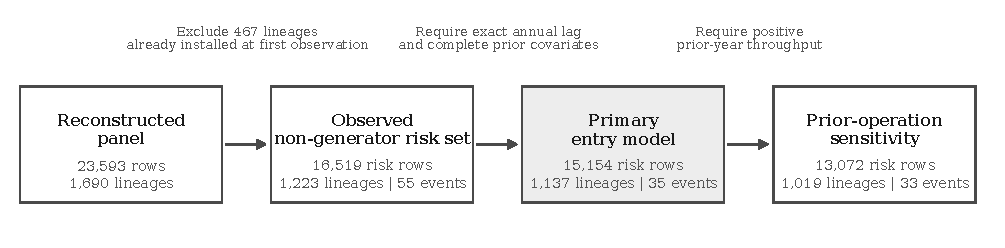
\includegraphics[width=\textwidth,height=0.72\textheight,
  keepaspectratio]{figure_entry_sample_flow.pdf}
\caption[Entry-model sample construction]{Entry-model sample construction. The reconstructed panel contains
23,593 facility-years from 1,690 administrative lineages. Restricting attention
to lineages first observed without positive installed capacity produces 16,519
risk rows and 55 observed entries; exact annual lags and complete prior
covariates define the 15,154-row, 35-event primary model. The prior-operation
sensitivity further requires positive prior-year throughput. The 467 lineages
already installed at first observation are left-censored, not non-adopters.}
\label{fig:entry-flow}
\end{figure}

The entry sample excludes 467 lineages already reporting positive installed
capacity in their first observed year because their entry time is left-censored.
A remaining lineage contributes annual risk rows until its first positive
capacity observation or its last observed non-generating year. The first
observed risk row is dropped from modeling because a lagged predictor is not
available. The complete-covariate frame further drops 120 rows with missing
lagged age or processing capacity, and 22 non-adjacent rows are excluded from
the exact-year model; none of those 22 rows contains an event.

The 55 descriptive events, the 35 complete-covariate events, and the pathway
categories answer different bookkeeping questions. Coincidentally, the pathway
audit also identifies 35 continuity-lineage events. That count should not be
conflated with the 35 events in the exact-year regression sample. The former is
a pathway classification among observed entries; the latter is a covariate
completeness restriction.

\subsection{RQ1: coverage definitions and fleet composition}

The first research question compares four transparent percentages rather
than asking readers to follow several similar formulas. Facility participation
is the percentage of retained records reporting positive installed electrical
capacity. The active-facility version uses only records with positive annual
throughput in the denominator. Throughput coverage is the share of recorded
waste processed at facilities reporting positive electricity output. Design-
capacity coverage is the share of national waste-processing capacity located at
facilities reporting positive installed electrical capacity.

These measures answer different questions. Facility participation shows how
widely generation equipment appears across records, whereas throughput and
design-capacity coverage show how much waste activity or nominal processing
capacity lies within the generating segment. Positive output is used for the
throughput numerator because installed equipment does not guarantee generation
in every year.

The annual percentages are repeated cross-sections, not direct conversion rates
for continuing facilities. The analysis therefore repeats the FY2005 and FY2024
comparison among administrative lineages observed in both endpoint years, then
applies stricter same-episode and complete-panel checks. Endpoint-only groups
describe changes in observed fleet composition, but administrative appearance
or disappearance is not treated as verified physical opening or closure. The
formal definitions and accounting expressions are consolidated in Appendix B.

\subsection{RQ2: sparse first-entry model}

\subsubsection{Event and population at risk}

In plain terms, each eligible non-generator lineage contributes one row for
each year in which it remains observed and has not previously reported positive
installed capacity. The outcome records whether that lineage first reports
positive capacity in the current year. This structure compares entry profiles
among lineages that could still experience a first observed entry; it does not
compare all facilities indiscriminately.

The event is the first observed year with positive installed electrical capacity
after a lineage has been observed without it. It is an administrative state
transition. It does not uniquely identify first physical operation, equipment
installation, or a particular construction history.

Positive installed capacity means a non-missing reported value greater than
zero. A blank or zero field means no reported positive capacity; it is not
verified physical absence. In total, 49 panel rows across 6 lineages report
positive gross output with blank or zero installed capacity. None of the 35
modeled events reports positive output in its immediately prior year, and 32
report positive output in the event year. A stricter sensitivity requires two
observed prior years with neither positive reported capacity nor output; it
retains 14,000 rows, 1,110 lineages, and 30 events.

\subsubsection{Primary model, estimator, and uncertainty}

The model asks a narrow question: among lineages still at risk, how do the odds
of first reported entry vary with prior-year age and processing scale after
accounting for calendar time and elapsed observed time at risk? It describes
those profiles; it does not estimate what would happen if a municipality
physically enlarged or aged a facility.

Discrete-time event-history analysis represents each at-risk lineage-year as a
binary outcome (Allison, 1982; Beck et al., 1998). For lineage $i$ in year
$t$, let $H_{it}=1$ indicate that the lineage remains in the first-entry risk
set at the start of the year because no earlier observed year reported positive
installed capacity. The primary model is

\begin{equation}
\begin{aligned}
\operatorname{logit}\!\left\{\Pr(Y_{it}=1\mid H_{it}=1)\right\}
&=\alpha+\beta_A\frac{A_{i,t-1}}{10}
+\beta_C\log\!\left(1+\frac{C_{i,t-1}}{100}\right) \\
&\quad+\beta_T\frac{t-2014.5}{5}
+\beta_R\log(1+R_{it}).
\end{aligned}
\label{eq:entry-model}
\end{equation}

Here, $Y_{it}=1$ denotes first reported positive installed capacity, $A$ is
prior-year reported age, $C$ is prior-year processing design capacity, and
$R$ is elapsed observed time at risk. Processing capacity is measured in tonnes
per day (t/day). Age is scaled per ten years and calendar time per five years.
Including the intercept, the model has five
parameters for 35 broad-frame events. The five-parameter specification was selected to remain proportionate to the 35 available events. An expanded 11-parameter model is retained as a sensitivity rather than treated as the primary model. Technology and geography
are not added because 35 events cannot support a larger adjustment set reliably.
Their omission is a limitation: processing scale can absorb unobserved
technology, regional, financial, or municipal differences. Leave-one-prefecture
fits assess concentration and influence only; they are not geographic-
confounding control.

With only 35 modeled events, ordinary maximum-likelihood logistic regression can be biased or produce unstable estimates when predictors nearly separate events from non-events. Firth logistic regression is therefore used because it reduces small-sample bias and retains finite estimates under separation (Firth, 1993; Heinze \& Schemper, 2002). Uncertainty is evaluated with 1,999 cluster-bootstrap replications that resample complete administrative lineages, preserving repeated observations from the same lineage. The penalized likelihood is shown in Appendix B.

Four frames are fitted. The broad exact-year frame is primary and includes every complete
at-risk row whose lag belongs to the same stable administrative lineage; it can
cross an inferred asset-episode boundary because its estimand is first
administrative-lineage entry. The prior-operation frame is a nested sensitivity
that additionally requires positive prior-year throughput. It is not an
independent comparison group, so differences between it and the broad frame are
not treated as an equality or equivalence test. A same-asset-episode continuity
sensitivity excludes the 59 exact-year rows that cross an inferred episode
boundary, including 11 events. An identity-certain sensitivity excludes every
lineage containing any of the 16 accepted uncertain links. The prior-operation,
same-asset-episode, and identity-certain frames are sensitivity analyses rather
than co-primary models.

\subsubsection{Translating the scale association}

Odds ratios show relative differences but can obscure how rare entry remains.
The thesis therefore reports both the predefined 300-versus-100 t/day
odds ratio and standardized annual risks at scale values with substantially
greater empirical support.

The 300-versus-100 t/day odds ratio is calculated from the fitted processing-scale coefficient. To show that entry remains uncommon in absolute terms, fitted annual probabilities are also averaged over the observed distributions of age, calendar year, and elapsed risk. This standardization changes only the capacity value while retaining the other observed predictors. The resulting values are adjusted descriptions of the observed risk population, not effects of physically enlarging a facility. Appendix B gives the formulas.

The 300-versus-100 contrast is retained as an upper-tail sensitivity comparison, and its limited empirical support is made explicit. In the broad risk frame, 24,
60, and 120 t/day are the 25th percentile, median, and 75th percentile; 300
t/day is approximately the 99th empirical percentile. Only 315 of 15,154 risk
rows and four of 35 events occur at or above 300 t/day. Annual risk is therefore
also standardized at 24, 60, and 120 t/day to display the fitted gradient in
denser regions of the data.

\subsubsection{Sensitivity and design diagnostics}

The remaining checks ask whether the scale profile depends on continuity,
reporting-state, functional-form, or geographic-concentration choices. They
test fragility; they do not convert the association into a causal effect.

The expanded 11-parameter Firth model and conventional links remain
specification sensitivities.

Three additional diagnostics retain the same five-parameter structure. The
capacity term is replaced by either $\log(1+C)$ or linear $C/100$ and translated
to its own 300-versus-100 t/day contrast. The model is also refitted after
omitting each of the 21 prefectures containing an event, and on the
two-prior-year reporting-state frame. These diagnostics use model-based
intervals; they test functional-form, geographic, and state-definition fragility
but do not replace the 1,999-lineage-bootstrap primary inference.

Finally, a design audit reports predictor correlations and variance inflation
factors (VIFs). Calendar time and logged elapsed risk are correlated because a
lineage observed for longer also tends to appear later in the panel. The audit
therefore limits interpretation of those temporal coefficients and checks
whether that dependence extends to the processing-scale term. The flexible
calendar-era and duration-band model remains the corresponding specification
sensitivity.

\subsection{RQ3: engineering decomposition and component models}

\subsubsection{Quantities and analysis sample}

This section proceeds in two steps. First, it models installed generator size
and annual use as separate outcomes. Second, it uses an exact accounting
identity to show how those components combine with waste loading to produce
gross MWh/t. The identity organizes interpretation; it is not a second source
of empirical evidence.

The engineering analysis separates what is installed from how intensively it is
used. Let $G_{it}$ be annual gross generation in megawatt-hours (MWh), $W_{it}$
annual throughput in tonnes, $K_{it}$ installed electrical capacity in
kilowatts (kW), and $C_{it}$ waste-processing design capacity in tonnes per day
(t/day). Define

\begin{align}
Y_{it}&=\frac{G_{it}}{W_{it}}
&&\text{(gross generation intensity, MWh/t)},
\label{eq:gross-intensity}\\
D_{it}&=\frac{K_{it}}{C_{it}}
&&\text{(generator design intensity, kW per t/day)},
\label{eq:design-intensity}\\
F_{it}&=\frac{G_{it}}{8.76K_{it}}
&&\text{(annual electrical capacity factor)},
\label{eq:capacity-factor}\\
U_{it}&=\frac{W_{it}}{365C_{it}}
&&\text{(waste-processing utilization)}.
\label{eq:waste-utilization}
\end{align}

The factor 8.76 converts one kW operating for 8,760 hours into annual MWh. These
quantities come from annual administrative reports rather than continuous meter
or dispatch records. Accordingly, this thesis treats $F_{it}$ as an
administrative annual electrical capacity-factor proxy; later references to
``capacity factor'' use this bounded meaning. The definitions imply the exact
facility-year identity

\begin{equation}
Y_{it}=\frac{8.76}{365}\frac{D_{it}F_{it}}{U_{it}}
=0.024\frac{D_{it}F_{it}}{U_{it}}.
\label{eq:engineering-identity}
\end{equation}

Gross MWh/t is thus a ratio produced jointly by installed sizing, annual use of
that electrical capacity, and annual waste loading. The identity does not say
that any one component is exogenous. For example, throughput, capacity factor,
maintenance, and waste composition may be jointly determined during a year.

The primary sample requires positive installed capacity, throughput, and gross
output. Values are excluded rather than clipped if gross intensity falls
outside 0.01--0.80 MWh/t, electrical capacity factor outside 0.02--1.20,
waste-processing utilization outside 0.02--1.20, or generator design intensity
outside 0.1--100 kW per t/day. A non-missing non-negative reported age and all
model fields are also required. Of 6,660 positive-throughput, positive-output
rows, 149 fail at least one check, leaving 6,511 rows across 493 lineages.
Heating value between 3 and 25 megajoules per kilogram (MJ/kg) is audited as a
plausibility field but is not an inclusion condition for the primary component
models; 102 otherwise valid rows lack it.

These thresholds are broad plausibility screens, not engineering-performance
standards and not cut points selected to optimize the reported estimates. The
lower bounds remove zeros and near-zero ratios inconsistent with the intended
operating-generator-year frame. The 1.20 upper bounds for capacity factor and
waste utilization deliberately allow moderate calendar, reporting, and
denominator mismatch instead of treating 1.00 as an error-free physical ceiling.
Only 5 of 6,511 retained capacity-factor rows exceed 1.00, and the principal
component conclusions remain stable under the conservative-bound sensitivity.
The wide design-intensity range permits heterogeneous generator sizing while
removing ratios likely driven by unit or field errors. Conservative and broad
predefined-bound sensitivities test dependence on these choices; unusual valid
observations may still be excluded, and plausible-looking errors may remain.

\subsubsection{Primary component models}

The first pair of models asks whether reported start-year cohorts differ in raw
installed generator size and annual electrical-capacity use after comparing
records with the same observed scale, technology, furnace count, and fiscal
year. Keeping these outcomes separate prevents gross MWh/t from acting as an
ambiguous stand-alone performance score.

Two pooled ordinary-least-squares models are estimated with standard errors clustered by administrative lineage (Wooldridge, 2010). The first models reported installed electrical capacity after adjustment for processing scale, start-year cohort, furnace count, technology groups, and fiscal year. The second models annual electrical capacity factor with the same adjustment set plus waste-processing utilization. The 2010-or-later start-year cohort is the reference group. Reported facility start year is an administrative cohort marker, not a verified generator-installation date. A separate gross-output model relates reported generation to annual throughput and installed capacity under the same cohort, technology, furnace-count, and year adjustments. Appendix B gives the full specifications.

\subsubsection{Common-control accounting decomposition}

This second step is an accounting reconciliation rather than another
performance test. By applying exactly the same rows and controls to every
component, it allocates each adjusted gross-intensity contrast among installed
sizing, annual electrical-capacity use, and waste loading.

Four additional regressions use exactly the same rows and control variables for generator design intensity, capacity factor, waste utilization, and gross generation intensity. Because the four outcomes are algebraically connected, each adjusted gross-intensity cohort gap equals the generator-design component plus the capacity-factor component minus the waste-utilization component. Appendix B reports the formal regression system.

This common-control identity decomposition is an accounting reconciliation of
the relative log-scale components of generator sizing, annual electrical-
capacity use, and waste loading. Because the equality is guaranteed by the
definitions and identical regression design matrices, it cannot independently
confirm the outcome models or establish causal mediation. It is distinct from
the primary capacity-factor model above, which
includes $U$ and asks how capacity factor differs at equal observed waste
utilization. Those conditional capacity-factor coefficients cannot be inserted
into the component sum. A sensitivity excludes the 14 lineages whose reported
facility start-year cohort changes during follow-up, leaving 6,291 rows across 479
lineages.

\subsubsection{Diagnostics, robustness, and exploratory extension}

These checks examine whether the component interpretation survives alternative
samples, bounds, time periods, and within-episode comparisons. The final
pathway comparison remains exploratory because observed administrative labels
cannot identify physical project mechanisms.

A specification diagnostic compares a baseline regression of $\log Y$ on
reported age, processing scale, waste utilization, heating value, technology,
and year with the same model after adding $\log D$. Both specifications use the
5,806 engineering-valid rows with reported heating value in the 3--25 MJ/kg
plausibility range. This is not a causal mediation design. It asks whether
coefficients previously attributed to age, scale, or utilization are stable
after the omitted installed-sizing component is represented.

Robustness checks split the period into FY2005--FY2014 and FY2015--FY2024, give
each lineage equal total weight, and apply conservative and broad predefined
engineering bounds. Asset-episode fixed effects and exact-adjacent first
differences are used only for operating components that vary meaningfully
within an episode. Design intensity is predominantly a between-asset attribute,
so within-episode change is not presented as its primary estimand.

Finally, event pathways are classified from observed administrative continuity.
A continuity-lineage entry remains in the same lineage and asset episode across
adjacent years without a reported reset. A rebuild/replacement-like entry has an
asset-episode, reported-start-year, or mature-to-new age reset. A
forward-dated/placeholder entry has a future start year or new-build placeholder
name. These labels are descriptive evidence rules. They do not verify the
physical project mechanism. First-complete-year outcomes are compared as
within-fiscal-year percentile ranks among engineering-valid generators, which
reduces confounding by fleet-wide time trends but does not remove selection into
each pathway.

\section{Results}

The results follow the three analytical populations defined in
Table~\ref{tab:frames}. In this section, \emph{entry} always means first reported
positive installed capacity within an observed administrative lineage, and
gross MWh/t remains a composite gross-output ratio rather than an independent
efficiency measure.

\subsection{RQ1: facility counts understate waste-volume coverage}

\noindent\textbf{Answer first.} Count-based participation understates the share
of observed waste activity covered by generating facilities, while the much
smaller change among endpoint-common lineages shows that the all-record trend
should not be read as widespread conversion among continuing facilities.

The official 415/991 ratio (41.9\%) describes the Ministry's published count of
electricity-generating facilities. The results below use the separate analytical
definition of positive installed capacity among retained facility records.

Installed-capacity participation rises steadily from 21.6\% of facility records
in FY2005 to 41.1\% in FY2024. Positive-output facilities already handle a much
larger share of waste: throughput coverage rises from 60.5\% to 80.1\% over the
same period. The design-capacity share at installed-capacity facilities moves
from 56.0\% to 70.5\%. Figure~\ref{fig:coverage} therefore shows long-run
increases with year-to-year variation under all three denominators, alongside a
persistent count-volume gap.

The lineage diagnostic changes the interpretation of that 19.50-percentage-
point rise. Among 732 administrative lineages observed in both FY2005 and
FY2024, installed-capacity prevalence increases only from 29.92\% to 32.10\%,
or 2.19 points. Among 678 endpoint-common lineages retaining the same reported
asset episode, it increases from 30.53\% to 31.42\%, or 0.88 points. The 713
lineages observed in all 20 fiscal years show a similarly modest change, from
29.73\% to 32.26\%.

\begin{table}[!htbp]
\centering
\caption{Endpoint fleet-composition diagnostic}
\label{tab:endpoint-composition}
\small
\setlength{\tabcolsep}{4pt}
\renewcommand{\arraystretch}{1.08}
\begin{tabularx}{\textwidth}{Y R{0.9cm} R{1.25cm} R{1.65cm} R{1.2cm}}
\toprule
Administrative group & FY & $N$ & With capacity & Share \\
\midrule
All endpoint records & 2005 & 1,318 & 285 & 21.62\% \\
All endpoint records & 2024 & 1,014 & 417 & 41.12\% \\
Endpoint-common lineages & 2005 & 732 & 219 & 29.92\% \\
Endpoint-common lineages & 2024 & 732 & 235 & 32.10\% \\
Endpoint-common, same episode & 2005 & 678 & 207 & 30.53\% \\
Endpoint-common, same episode & 2024 & 678 & 213 & 31.42\% \\
FY2005-only lineages & 2005 & 586 & 66 & 11.26\% \\
FY2024-only lineages & 2024 & 282 & 182 & 64.54\% \\
\bottomrule
\end{tabularx}
\renewcommand{\arraystretch}{1}
\normalsize
\end{table}

The endpoint-only groups are sharply different: 64.54\% of FY2024-only
lineages report installed capacity, compared with 11.26\% of FY2005-only
lineages. Together with the much smaller endpoint-common increase, this pattern
is consistent with a substantial contribution from changing observed fleet
composition rather than widespread conversion among continuing lineages. It is
not an additive decomposition and does not identify physical construction or closure because
administrative appearance and disappearance can also reflect reporting and
identity history.

The FY2024 cross-section makes the distinction concrete. The administrative
panel contains 1,014 facility records, of which 417 report positive installed
electrical capacity, giving the 41.1\% all-record participation rate. Among the
879 records with positive throughput, 408 report installed capacity, or 46.4\%.
Holding the installed-capacity state fixed therefore isolates a 5.3-percentage-
point denominator difference. Positive output appears in 410 records: 40.4\% of
all records and 46.6\% of positive-throughput records. The two output percentages
use the same numerator state and isolate a 6.2-point denominator difference.

The 410 positive-output facilities process 24.70 million of the 30.84 million
recorded tonnes, or 80.1\%. In contrast, 469 operating non-generators process
6.14 million tonnes, or 19.9\%. Another 126 records report neither positive
throughput nor generation, and nine installed-capacity records report no
positive output. Two FY2024 records report positive output without positive
installed capacity. Installed-capacity and positive-output states are therefore
reported separately rather than forced into one binary partition.

After the predefined output and capacity-factor checks, valid generator rows
cover 79.7\% of FY2024 throughput. Their throughput-weighted conditional gross
intensity is 0.425 MWh/t. Multiplying 0.797 by 0.425 gives 0.338 MWh per total
fleet tonne, exactly matching valid gross generation divided by all recorded
throughput. This arithmetic is more informative than the facility count alone:
most recorded waste is already processed at facilities reporting positive
generation, even though installed equipment appears in fewer than half of
facility records.

The result does not imply that the remaining 19.9\% of operating throughput can
or should all be redirected or equipped. It also does not measure electricity
used internally, net export, heat recovery, marginal emissions, or project
cost. Its contribution is denominator discipline: installed-capacity
participation is 41.1\% among all records and 46.4\% among active records, while
positive-output participation is 40.4\% and 46.6\%, respectively. Positive-
output facilities cover 80.1\% of tonnes, and installed-capacity facilities
cover 70.5\% of design capacity. Matching on activity narrows the count-volume
contrast but does not remove it.

\subsection{RQ2: entry is rare and associated with processing scale}

\noindent\textbf{Answer first.} First reported entry remains uncommon across
the observed risk set, but its positive association with prior-year processing
scale is stable across the reported sensitivity analyses. The age profile is
less stable across continuity definitions and does not support an age-only
rule.

The descriptive risk set contains 55 first reported installed-capacity entries.
The 35 exact-year modeled events comprise 24 continuity-lineage and 11
rebuild/replacement-like entries; none is forward-dated. The four calendar eras
contain 7, 4, 14, and 10 modeled events, respectively.

Only 35 events remain after requiring an exact one-year lag and complete prior
age and capacity; 33 remain after requiring positive prior-year throughput.
This sparse count is central to interpretation. The Firth model addresses
finite-estimate and first-order bias problems, but it cannot create information
that the panel does not contain.

Observed rates already show strong scale ordering. Entry occurs in 1 of 3,854
risk rows in the smallest processing-capacity quartile (0.026\%), 2 of 4,175 in
the second quartile (0.048\%), 9 of 3,702 in the third (0.243\%), and 23 of 3,423
in the largest (0.672\%). Because risk duration, calendar period, and age differ
across these groups, the adjusted model is needed before interpreting the
gradient.

The most defensible translation begins where observations are dense. At the
risk-frame 25th percentile, median, and 75th percentile of 24, 60, and 120
t/day, standardized annual predictions are 0.68 (95\% confidence interval [CI]
0.35--1.08), 1.37
(0.84--1.97), and 3.29 (2.28--4.57) entries per 1,000 facility-years. The 100
t/day comparison level gives 2.53 (1.73--3.52). Entry is uncommon
throughout this support-rich range, but the fitted absolute risk rises with
processing scale.

The primary five-parameter broad Firth model gives a coefficient of 2.749 on
$\log(1+C/100)$. Its retained 300-versus-100 t/day contrast has an odds ratio of
6.72 with a 1,999-lineage-bootstrap 95\% CI of 4.31--12.46. The standardized
predictions are 2.53 and 16.66 entries per 1,000 facility-years, a difference of
14.13 (7.38--26.77). The 300 t/day value is an upper-tail prediction at the 98.98th
empirical percentile: only 315 rows (2.08\%) and 4 modeled events occur at or
above it. It is retained as a predefined upper-tail sensitivity contrast, not
treated as the only or most representative translation of the model.

The prior-operation, same-episode, and identity-certain 300-versus-100 odds
ratios are 7.09 (4.08--13.76), 7.15 (4.44--14.05), and 6.76 (4.23--12.30),
respectively. Because these frames are nested, their coefficients are parallel
sensitivity estimates rather than between-group contrasts.

The broad age coefficient is -0.327 per ten years (bootstrap CI -0.774 to
0.070); prior-operation and identity-certain intervals also span zero. The
same-episode estimate is -0.751 (CI -1.364 to -0.206) but uses only 24 events.
Age is therefore continuity-sensitive. Reclassifying each event leaves scale
odds ratios from 6.12 to 7.30; deleting each event's entire lineage leaves 6.13
to 7.30. No one event or event lineage creates the scale result.

Alternative capacity forms also remain positive. Using $\log(1+C)$ gives an
odds ratio of 5.01 (model-based 95\% CI 2.85--8.83), while linear capacity gives 4.22
(2.69--6.61). Omitting each event prefecture gives 6.14--7.18 across 21 fits.
The stricter 30-event reporting-state frame gives 6.21 (3.26--11.81). These are
diagnostics with model-based intervals; only the primary uses the
1,999-lineage bootstrap for headline uncertainty.

The design audit gives a correlation of 0.909 between calendar time and logged
elapsed risk. Their VIFs are 5.76 and 6.15, so those temporal coefficients are
not interpreted separately. The processing-scale VIF is only 1.10, and its
correlations with calendar time and elapsed risk are 0.013 and 0.039. Temporal
dependence therefore qualifies the nuisance time terms but does not explain the
estimated scale ordering. The flexible era/duration sensitivity yields a
similar 300-versus-100 odds ratio of 6.13.

\begin{table}[!htbp]
\centering
\caption{Consolidated entry specification audit}
\label{tab:entry-specifications}
\scriptsize
\setlength{\tabcolsep}{3.1pt}
\renewcommand{\arraystretch}{1.13}
\begin{tabularx}{\textwidth}{L{3.15cm}R{1.25cm}L{2.45cm}Y}
\toprule
Specification & Events or fits & 300-versus-100 t/day odds ratio & Purpose and inference \\
\midrule
Primary five-parameter broad frame & 35 & 6.72 (4.31--12.46) & Primary;
1,999-lineage bootstrap \\
Prior-operation frame & 33 & 7.09 (4.08--13.76) & Positive prior-year throughput \\
Same-episode frame & 24 & 7.15 (4.44--14.05) & Episode-boundary continuity \\
Identity-certain frame & 35 & 6.76 (4.23--12.30) & Uncertain-link exclusion \\
Flexible era/duration Firth model & 35 & 6.13 (3.92--11.21) & 11-parameter
temporal-form check; 499 whole-lineage bootstrap replications \\
Alternative capacity forms & 2 fits & 4.22--5.01 & Functional form;
model-based lower CI bounds 2.69--2.85 \\
Two-prior-year reporting state & 30 & 6.21 (3.26--11.81) & Stricter prior-state evidence \\
Leave-one-event-prefecture fits & 21 fits & 6.14--7.18 & Geographic influence,
not confounding control \\
Event or event-lineage attacks & 70 fits & 6.12--7.30 & Single-event influence \\
\bottomrule
\end{tabularx}
\renewcommand{\arraystretch}{1}
\normalsize
\end{table}

Table~\ref{tab:entry-specifications} distinguishes bootstrap headline inference
from model-based and deletion diagnostics. A stable direction across these rows
does not recover unobserved technology, finance, policy exposure, or project
history omitted from the model.

\begin{figure}[H]
\centering
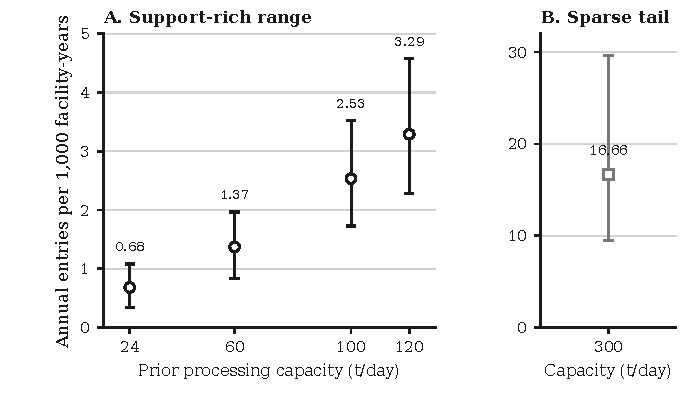
\includegraphics[width=0.80\textwidth,height=0.72\textheight,
  keepaspectratio]{thesis_entry_support.pdf}
\caption[Standardized first-entry risk by prior processing capacity]{Standardized annual first-entry risk from the five-parameter Firth
logistic model, expressed as entries per 1,000 facility-years at specified
prior-year processing capacities. Points are model-standardized predictions;
vertical bars are 95\% intervals from 1,999 whole-lineage bootstrap
replications. Panel A shows the support-rich 24--120 t/day range. Panel B uses a
different vertical scale to isolate the 300 t/day prediction; 300 t/day is the
98.98th percentile, with only 315 risk rows and four events at or above that
level.}
\label{fig:entry}
\end{figure}

The supported RQ2 conclusion is narrow and stable across the reported
sensitivities. First reported capacity entry is rare and positively associated
with processing scale. This concerns witnessed
transitions among prior non-generators, not entry across the whole fleet. The
administrative data do not establish a general independent age pattern, and
scale can proxy for contracts, finances, catchments, technology, geography, or
municipal capacity. Neither profile should be used as if the model had
identified an equipment-project response.

\FloatBarrier
\subsection{RQ3: cohort differences show a substantial installed-sizing component}

\noindent\textbf{Answer first.} Reported start-year cohorts differ much more
clearly in installed generator size than in uniformly lower annual electrical-
capacity use. Gross MWh/t therefore cannot distinguish design from operation
unless its components are analyzed separately.

The engineering-valid generator frame has 6,511 observations from 493 stable
lineages. Median gross intensity is 0.327 MWh/t, median generator design
intensity is 14.0 kW per t/day, median electrical capacity factor is 0.607, and
median waste-processing utilization is 0.609. These summaries describe
generator-years that pass stated bounds, not the full fleet.

The RQ3 conclusion rests first on separate raw installed-kW and annual capacity-
factor models. The exact component identity then explains how those independently
reported quantities combine; it is not treated as independent evidence that
sizing must dominate.

Reported facility start-year cohorts differ much more in installed generator
size than in annual capacity factor. Relative to 2010 or later and conditional on observed
controls, adjusted installed capacity is 79.1\% lower before 1990, 58.6\% lower
in 1990--1999, and 23.5\% lower in 2000--2009.

The installed-kW elasticity with respect to processing t/day is 1.532 (95\% CI
1.447--1.617), and the coefficient of determination ($R^2$) is 0.786.
Subtracting one gives the 0.532
design-intensity elasticity under identical controls; this is algebraic rather
than independent replication.

The electrical-capacity-factor model tells a different story. Conditional on
processing scale, waste utilization, technology, furnace count, and fiscal
year, pre-1990 and 1990s capacity factors are 35.3\% (95\% CI 24.6--46.8\%) and
22.0\% (14.4--30.0\%) higher. The 2000s estimate is 1.5\% higher, with a CI from
4.1\% lower to 7.4\% higher. Waste
utilization is positively associated with log electrical capacity factor
(coefficient 1.695, 95\% CI 1.448 to 1.942), while processing scale is negatively
associated (-0.116, 95\% CI -0.162 to -0.070). This model explains 33.9\% of log
capacity-factor variation. These coefficients describe annual use of installed
kW. They do not show that utilization has an independent positive association
with gross MWh/t after generator sizing is represented.

The common-control decomposition provides a narrower accounting reconciliation.
Every row in Table~\ref{tab:common-control} uses the same 6,511 observations and
the same cohort, processing-scale, technology, furnace-count, and year controls.
The three component columns are log differences from the 2010-or-later cohort
and sum exactly to the directly fitted log gross-intensity difference.

\begin{table}[!htbp]
\centering
\caption{Common-control cohort decomposition of log gross MWh/t}
\label{tab:common-control}
\small
\setlength{\tabcolsep}{3.5pt}
\renewcommand{\arraystretch}{1.12}
\begin{tabularx}{\textwidth}{L{2.4cm} C C C C}
\toprule
Cohort & Design $\gamma_D$ & Capacity factor $\gamma_F$ & Waste loading $-\gamma_U$ & Total $\gamma_Y$ \\
\midrule
Before 1990 & -1.565 & +0.016 & +0.299 & -1.250 \\
1990--1999 & -0.883 & +0.020 & +0.172 & -0.690 \\
2000--2009 & -0.267 & -0.094 & +0.089 & -0.272 \\
\bottomrule
\end{tabularx}
\renewcommand{\arraystretch}{1}
\normalsize
\end{table}

Installed sizing is the largest absolute point-estimate accounting component in
every older cohort. For
the pre-1990 and 1990s cohorts, common-control capacity-factor differences are
near zero; their positive capacity-factor coefficients in the primary model
arise after conditioning on waste utilization and answer a different equal-
utilization question. For the 2000s cohort, both smaller sizing and a lower
common-control capacity factor contribute. Excluding all 14 cohort-switching
lineages leaves 6,291 rows across 479 lineages and produces the same ordering,
with direct log gaps of -1.306, -0.702, and -0.280. These exact conditional
sums are accounting attribution, not causal mediation.

\begin{figure}[!htbp]
\centering
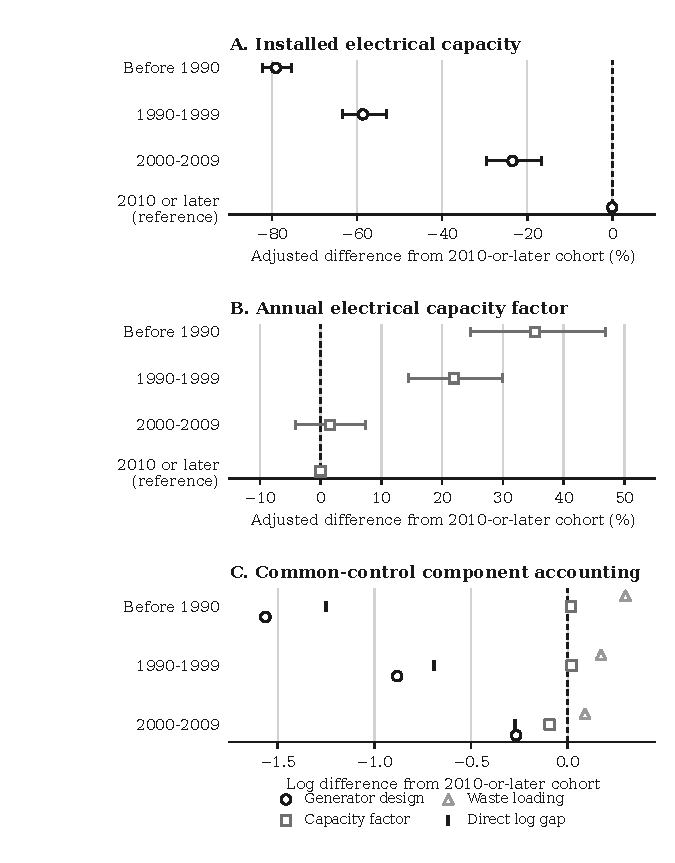
\includegraphics[width=0.78\textwidth,height=0.72\textheight,
  keepaspectratio]{thesis_cohort_components.pdf}
\caption[Reported start-year cohort models and component accounting]{Reported facility start-year cohort evidence for 6,511
engineering-valid facility-years from 493 administrative lineages. Panels A
and B show adjusted percentage differences from the 2010-or-later cohort in
installed electrical capacity and annual electrical capacity factor; bars are
lineage-clustered 95\% confidence intervals. Panel C uses the same sample and
common controls to reconcile the direct log gross-MWh/t gap into generator
design, capacity-factor, and waste-loading components. Those components sum by
an exact accounting identity and do not estimate causal mediation. Reported
facility start year is not a verified generator-installation date.}
\label{fig:components}
\end{figure}

The direct gross-output model is consistent with the component structure. The
elasticity of annual gross MWh with respect to throughput is 0.638 (95\% CI
0.536 to 0.740), and the elasticity with respect to installed electrical
capacity is 0.576 (95\% CI 0.502 to 0.650), conditional on cohort, observed
technology, furnace count, and year. The model $R^2$ is 0.914. It shows that
both waste loading and installed kW are associated with annual output, but it is not
a production function with exogenous inputs.

An accounting-consistency diagnostic compares gross-intensity specifications on
the 5,806-row plausible-heating-value subset. In the baseline model without
generator design intensity, the reported-age coefficient is -0.0349, the
processing-capacity coefficient is 0.1001, and the waste-utilization coefficient
is 0.6699; all have $p<0.001$. After adding log generator design intensity, the
corresponding coefficients become -0.0020 ($p=0.2977$), -0.0092
($p=0.1991$), and -0.0995 ($p=0.2038$). The sizing coefficient is 0.7532
($p<0.001$), and model $R^2$ rises from 0.4737 to 0.8131. This is not a causal
decomposition, and the increase is partly expected because design intensity is
algebraically related to gross MWh/t. The diagnostic shows that the former age,
scale, and utilization interpretation is sensitive to whether installed sizing
is represented; it does not independently prove that sizing causes the cohort
pattern.

Adjacent-year rank persistence is highest for generator design intensity:
0.995 across 5,963 pairs from 470 lineages. Gross-intensity rank persistence is
0.961 and capacity-factor persistence is 0.873. The corresponding within-to-total
variance ratios are 0.016 for log design intensity, 0.089 for log gross
intensity, and 0.426 for log capacity factor. Sizing is therefore mostly a
between-asset design attribute, while annual capacity factor contains much more
within-asset movement.

The principal component conclusions remain stable across the two ten-year
windows, lineage-equal weighting, and conservative or broad engineering bounds.
For example, the processing-scale coefficient in the design-intensity model is
0.474 in FY2005--FY2014 and 0.577 in FY2015--FY2024; it is 0.520 under
conservative bounds and 0.536 under broad bounds. Excluding every
identity-uncertain lineage leaves
6,450 rows across 487 lineages and gives a nearly unchanged coefficient of
0.533. Within-asset-episode models also retain a positive association between
utilization and electrical capacity factor. Those checks strengthen the
component description but do not resolve
simultaneous changes in throughput, maintenance, installed capacity, and output.

\section{Discussion}

\subsection{What the thesis changes in the fleet narrative}

Each analytical margin corrects a different intuitive but incomplete reading of
the fleet. Table~\ref{tab:interpretive-corrections} separates the tempting
interpretation from the strongest statement supported by the evidence.

\begin{table}[!htbp]
\centering
\caption{Interpretive corrections produced by the three-margin design}
\label{tab:interpretive-corrections}
\scriptsize
\setlength{\tabcolsep}{3.2pt}
\renewcommand{\arraystretch}{1.14}
\begin{tabularx}{\textwidth}{L{3.6cm}YY}
\toprule
Common reading & Evidence-based correction & Defensible interpretation \\
\midrule
Only about 41\% generate, so recovery reaches little waste. &
Positive-output facilities handle 80.1\% of throughput; installed-capacity
facilities represent 70.5\% of design capacity. &
Record prevalence is incomplete, but generation is concentrated in larger or
more active parts of the observed fleet. \\
The 19.50-point rise means widespread retrofit of incumbents. &
The rise is 2.19 points among 732 lineages observed at both endpoints. &
Changing observed composition is substantial, but the comparison is not an
additive decomposition and does not verify retrofit projects. \\
Newer cohorts are simply more efficient. &
Older cohorts have much smaller adjusted installed kW, but not uniformly lower
capacity factors; sizing is the largest absolute point-estimate component. &
Gross MWh/t combines sizing, annual capacity use, and waste loading; the
component identity is descriptive, not causal. \\
\bottomrule
\end{tabularx}
\renewcommand{\arraystretch}{1}
\normalsize
\end{table}

The transition model adds a separate correction. Processing scale is positively
associated with first reported entry in the primary model and all sensitivity
frames, but the model does not show that enlarging a facility would cause entry.
Scale can represent unobserved municipal, technical, and financial conditions.
Age is continuity-sensitive and therefore cannot support a simple age-only rule.

\subsection{Direct answers to the research questions}

\textbf{RQ1 is answered by matched state and denominator contrasts, not by one
preferred percentage.} In FY2024, positive-output facilities handle 80.1\% of
recorded throughput and installed-capacity facilities hold 70.5\% of processing
design capacity, despite installed capacity appearing in only 41.1\% of all
records. Generation is therefore concentrated in larger or more heavily used
parts of the observed fleet. The contrast does not mean that 80.1\% of waste
becomes electricity or that the covered facilities are environmentally optimal.
It also separates prevalence from incumbent diffusion: the all-record endpoint
increase is 19.50 percentage points, compared with 2.19 points among 732
lineages observed in both endpoint years.

\textbf{RQ2 is answered by a scale association stable across the reported
sensitivity analyses and a continuity-sensitive age association.} In the
support-rich 24--120 t/day range, standardized annual predictions rise from
0.68 to 3.29 entries per 1,000 facility-years. The primary
300-versus-100 t/day odds ratio is 6.72, and
Table~\ref{tab:entry-specifications} shows that the positive scale gradient
survives the continuity, functional-form, reporting-state, geographic, and
event-influence checks. The 300-t/day prediction is nevertheless a tail
contrast, supported by 315 risk rows and four events at or above that level.
Age is less stable across continuity definitions and should not support an
age-only screening rule. The outcome remains first reported positive installed
capacity within an administrative lineage, not a verified retrofit,
construction start, or causal response to changing capacity.

\textbf{RQ3 is answered by separating installed design from annual use.} Older
reported start-year cohorts have much smaller adjusted installed electrical
capacity, but not uniformly lower administrative capacity-factor proxies. Gross
MWh/t therefore combines generator sizing, annual capacity use, and waste
loading rather than acting as an independent operating-efficiency score. Under
shared controls, sizing is the largest absolute point-estimate accounting
component of every older-cohort gap. The exact component sum is reconciliation
by construction, not independent evidence, and the small pathway comparison
remains a hypothesis-generating appendix rather than an answer to RQ3.

Together, the answers provide one ordered diagnosis. RQ1 locates electricity
recovery within the fleet; RQ2 describes which observed non-generator lineages
first enter the installed-capacity state; and RQ3 explains the observable
structure inside the generating segment. No result is asked to answer a
question belonging to another frame. That separation is the central thesis
contribution and the main safeguard against an aggregate or conditional result
being interpreted causally.

\subsection{Evidence-bound implications}

Monitoring should report facility, throughput, and design-capacity coverage
together. Screening can treat processing scale as a marker for further
feasibility work, but not use an age-only rule. Observed generator-years that
meet the engineering-validity criteria should be compared conditional on sizing
and reported facility start-year cohort before gross MWh/t is interpreted as an
operating gap.

These are measurement and diagnostic implications, not a ranked list of
projects. The study does not determine whether a municipality should build,
replace, coordinate, maintain, or retire a facility. Such decisions require
capital costs, waste-supply agreements, grid and internal-use conditions,
maintenance history, emissions controls, heat demand, and alternatives higher
in the waste hierarchy. The thesis's role is to prevent an aggregate statistic
or misspecified ratio from deciding those questions implicitly.

\subsection{Limitations and next evidence needed}

The 20 workbooks are hash-identified and parser mappings are documented, but
their original retrieval timestamps and publisher-side revision history are
unavailable. Future acquisition should archive both.

Stable administrative lineages remain inferred. The resolver addresses exact
duplicates, code breaks, row-order dependence, and known difficult links, but no
physical-site registry verifies ownership, construction, or closure histories.
The blinded clerical-review packet is generated, but an independent reviewer has
not yet completed and adjudicated it. This outstanding validation step is
why the thesis describes deterministic linkage and sensitivity checks rather
than independently audited identity. Administrative absence is therefore not
modeled as a physical outcome.

Entry is rare and partially left-censored. Firth estimation and lineage
bootstrapping cannot overcome only 35 broad-frame, 33 prior-operation, and 24
same-episode events. Although all 1,999 requested bootstrap replications per
frame converge, resampling cannot create missing project information. The
parsimonious models omit financing, prices, contracts, catchments, maintenance,
and detailed technology. Scale may
proxy for these, so odds ratios are associations rather than effects of changing
t/day.

Installed-capacity state is also a reporting construct. Forty-nine panel rows
across six lineages report positive gross output despite a blank or zero
installed-capacity field. None is the immediately prior row of a modeled event,
and the two-prior-year sensitivity remains positive, but these checks do not
prove that blanks represent physical absence. External equipment or
commissioning records are needed to verify event meaning.

Generator fields also have strict boundaries. Gross generation is not net
export; on-site use and useful heat are incomplete; reported capacity may differ
from availability; and MWh/t is not the European Union R1 energy-efficiency
indicator, a lifecycle measure, or an economic measure (Grosso et al., 2010).
Heating-value coverage is insufficient for a common thermal measure. Bounds
remove 149 rows but may exclude unusual valid cases or retain plausible-looking
errors.

Reported facility start year is not an equipment date and can bundle original
design, later equipment, reporting, waste, and municipality context. Annual throughput,
capacity factor, maintenance, and output are jointly determined. Controls,
fixed effects, and adjacent differences do not create exogenous variation; the
equations remain accounting identities and conditional descriptions.

The 2010-or-later cohort enters only from FY2010 onward. Fiscal-year indicators
create within-year comparisons where cohorts overlap, but cannot remove
selective survival or unrecorded replacement.

The next evidence programme has three priorities. First, commissioning,
procurement, or equipment records should verify the 35 modeled events and the
administrative lineages around them. Second, net-export, internal-use, useful-
heat, outage, cost, and waste-composition records should characterize project
and operating performance. Third, only after policy exposure and credible
comparison units are observed should a later study attempt causal evaluation of
FIT, subsidy, retrofit, or replacement effects.

Finally, the pathway contrast is small and selected, and reported resets do not
verify physical replacement. It remains a hypothesis-generating pointer toward
the first and second evidence priorities, not a project-effect estimate.

\section{Conclusion}

Japan's fleet looks different at three margins. In FY2024, installed capacity
appears in 41.1\% of all records and 46.4\% of positive-throughput records;
positive output appears in 40.4\% and 46.6\%, respectively. Positive-output
facilities handle 80.1\% of throughput, and installed-capacity facilities
represent 70.5\% of processing design capacity. The 19.50-point all-record rise
since FY2005 is only 2.19 points among endpoint-common lineages, a contrast
consistent with a substantial fleet-composition contribution. At the transition
margin, standardized annual predictions rise from 0.68 to 3.29 entries per
1,000 facility-years across the support-rich 24--120 t/day range. The primary
300-versus-100 t/day odds ratio is 6.72, but 300 t/day is a thinly supported tail
contrast. The scale direction is stable across the reported sensitivity analyses, but age remains
continuity-sensitive and neither association is causal. At the component
margin, independent raw-kW and capacity-factor models show that cohort
differences are much larger for installed sizing than for uniformly lower annual
use. A shared-control identity then reconciles sizing as the largest absolute
point-estimate accounting component of each older-cohort gross-intensity gap; it
does not independently
confirm a causal mechanism.

The thesis's contribution is therefore not a claim that every non-generator is
an equal opportunity or that newer facilities simply perform better. It is a
three-margin diagnostic: reconstruct lineages before transitions, separate
counts from covered activity, and separate installed design from annual use.
That architecture gives readers a clear foundation for
deciding which next question requires engineering, capital-history, or causal
evidence.

\section*{Acknowledgements}

The author thanks Prof. Han Ji for supervision and critical feedback during the
development of this thesis.

\section*{References}
\addcontentsline{toc}{section}{References}
\begingroup
\small
\setlength{\parindent}{0pt}
\setlength{\parskip}{0.55em}

Agency for Natural Resources and Energy. (2017). \textit{FY2016 annual report on
energy: Outline}. Ministry of Economy, Trade and Industry.
\url{https://www.enecho.meti.go.jp/en/category/whitepaper/pdf/2017_outline.pdf}

Allison, P. D. (1982). Discrete-time methods for the analysis of event
histories. \textit{Sociological Methodology}, \textit{13}, 61--98.
\url{https://doi.org/10.2307/270718}

Astrup, T., M\o ller, J., \& Fruergaard, T. (2009). Incineration and
co-combustion of waste: Accounting of greenhouse gases and global warming
contributions. \textit{Waste Management \& Research}, \textit{27}(8), 789--799.
\url{https://doi.org/10.1177/0734242X09343774}

Astrup, T. F., Tonini, D., Turconi, R., \& Boldrin, A. (2015). Life cycle
assessment of thermal waste-to-energy technologies: Review and recommendations.
\textit{Waste Management}, \textit{37}, 104--115.
\url{https://doi.org/10.1016/j.wasman.2014.06.011}

Beck, N., Katz, J. N., \& Tucker, R. (1998). Taking time seriously:
Time-series-cross-section analysis with a binary dependent variable.
\textit{American Journal of Political Science}, \textit{42}(4), 1260--1288.
\url{https://doi.org/10.2307/2991857}

Brunner, P. H., \& Rechberger, H. (2015). Waste to energy -- key element for
sustainable waste management. \textit{Waste Management}, \textit{37}, 3--12.
\url{https://doi.org/10.1016/j.wasman.2014.02.003}

Chen, P.-C., Chang, C.-C., Yu, M.-M., \& Hsu, S.-H. (2012). Performance
measurement for incineration plants using multi-activity network data
envelopment analysis: The case of Taiwan. \textit{Journal of Environmental
Management}, \textit{93}(1), 95--103.
\url{https://doi.org/10.1016/j.jenvman.2011.08.011}

Cui, J., Cui, Y., Li, J., Gao, X., Wei, W., Chen, Y., Ma, W., Zhu, N., Geng,
Y., Zhao, Y., \& Lou, Z. (2026). Efficiency hierarchy and optimization of
waste incineration in China to balance disposal and energy supply.
\textit{Nature Communications}, \textit{17}(1), Article 3069.
\url{https://doi.org/10.1038/s41467-026-69897-w}

e-Stat. (n.d.). \textit{Nation Survey on the State of Discharge and Treatment
of Municipal Solid Waste} (Statistics code 00650101). Portal Site of Official
Statistics of Japan. \url{https://www.e-stat.go.jp/en/statistics/00650101}
(accessed 10 July 2026).

European Commission. (2017). \textit{The role of waste-to-energy in the
circular economy} (COM(2017) 34 final). European Commission.
\url{https://eur-lex.europa.eu/legal-content/EN/TXT/?uri=CELEX:52017DC0034}

Firth, D. (1993). Bias reduction of maximum likelihood estimates.
\textit{Biometrika}, \textit{80}(1), 27--38.
\url{https://doi.org/10.1093/biomet/80.1.27}

Geels, F. W. (2004). From sectoral systems of innovation to socio-technical
systems: Insights about dynamics and change from sociology and institutional
theory. \textit{Research Policy}, \textit{33}(6--7), 897--920.
\url{https://doi.org/10.1016/j.respol.2004.01.015}

Grosso, M., Motta, A., \& Rigamonti, L. (2010). Efficiency of energy recovery
from waste incineration, in the light of the new Waste Framework Directive.
\textit{Waste Management}, \textit{30}(7), 1238--1243.
\url{https://doi.org/10.1016/j.wasman.2010.02.036}

Han, Q.-l., Liu, H.-q., Gong, Y.-y., Tao, J.-y., Sun, Y.-n., Wei, G.-x., Zhu,
Y.-w., \& Chen, G.-y. (2025). Strengthening pollutant control and resource
recovery can enhance sustainable waste incineration in China.
\textit{Communications Earth \& Environment}, \textit{6}, Article 863.
\url{https://doi.org/10.1038/s43247-025-02859-0}

Harron, K., Doidge, J. C., \& Goldstein, H. (2020). Assessing data linkage
quality in cohort studies. \textit{Annals of Human Biology}, \textit{47}(2),
218--226. \url{https://doi.org/10.1080/03014460.2020.1742379}

Heinze, G., \& Schemper, M. (2002). A solution to the problem of separation in
logistic regression. \textit{Statistics in Medicine}, \textit{21}(16),
2409--2419. \url{https://doi.org/10.1002/sim.1047}

Liu, B., Wang, P., Zhou, J., Guo, Y., Ma, S., Chen, W.-Q., Li, J., \& Chang,
V. W.-C. (2025). Refocusing on effectiveness over expansion in urban
waste-energy-carbon development in China. \textit{Nature Energy}, \textit{10},
215--225. \url{https://doi.org/10.1038/s41560-024-01683-8}

Lombardi, L., Carnevale, E., \& Corti, A. (2015). A review of technologies and
performances of thermal treatment systems for energy recovery from waste.
\textit{Waste Management}, \textit{37}, 26--44.
\url{https://doi.org/10.1016/j.wasman.2014.11.010}

Ministry of the Environment Japan. (n.d.). \textit{High-efficiency waste power
generation facility development manual}. Ministry of the Environment Japan.
\url{https://www.env.go.jp/recycle/misc/he-wge_facil/} (accessed 17 July 2026).

Ministry of the Environment Japan. (2014). \textit{FY2014 waste-energy
introduction and low-carbon promotion project: Application guidelines}.
Ministry of the Environment Japan.
\url{https://www.env.go.jp/recycle/info/ondanka/kobo.html} (accessed 17 July
2026).

Ministry of the Environment Japan. (2026). \textit{General Waste Treatment
Survey results: FY2024 municipal solid waste treatment survey}. Environmental
Management Bureau, Ministry of the Environment Japan.
\url{https://www.env.go.jp/recycle/waste_tech/ippan/} (accessed 10 July 2026).

M\"{u}nster, M., \& Meibom, P. (2010). Long-term affected energy production of
waste to energy technologies identified by use of energy system analysis.
\textit{Waste Management}, \textit{30}(12), 2510--2519.
\url{https://doi.org/10.1016/j.wasman.2010.04.015}

Sakai, S., Ikematsu, T., Hirai, Y., \& Yoshida, H. (2008). Unit-charging
programs for municipal solid waste in Japan. \textit{Waste Management},
\textit{28}(12), 2815--2825.
\url{https://doi.org/10.1016/j.wasman.2008.07.010}

Sakai, S.-i., Yoshida, H., Hirai, Y., Asari, M., Takigami, H., Takahashi, S.,
Tomoda, K., Peeler, M. V., Wejchert, J., Schmid-Unterseh, T., Ravazzi Douvan,
A., Hathaway, R., Hylander, L. D., Fischer, C., Oh, G. J., Li, J., \& Chi, N. K.
(2011). International comparative study of 3R and waste management policy
developments. \textit{Journal of Material Cycles and Waste Management},
\textit{13}(2), 86--102.
\url{https://doi.org/10.1007/s10163-011-0009-x}

Sasao, T. (2018). How does municipal solid waste policy affect heat and
electricity produced by incinerators? \textit{Detritus}, \textit{2}, 133--141.
\url{https://doi.org/10.31025/2611-4135/2018.13650}

Seto, K. C., Davis, S. J., Mitchell, R. B., Stokes, E. C., Unruh, G., \&
\"{U}rge-Vorsatz, D. (2016). Carbon lock-in: Types, causes, and policy
implications. \textit{Annual Review of Environment and Resources},
\textit{41}(1), 425--452.
\url{https://doi.org/10.1146/annurev-environ-110615-085934}

Shino, Y. (2019). System analysis of MSW incinerator power generation
performance. \textit{Journal of the Japan Society of Material Cycles and Waste
Management}, \textit{30}, 113--121.
\url{https://doi.org/10.3985/jjsmcwm.30.113}

Sun, L., Fujii, M., Tasaki, T., Dong, H., \& Ohnishi, S. (2018). Improving
waste to energy rate by promoting an integrated municipal solid-waste
management system. \textit{Resources, Conservation and Recycling},
\textit{136}, 289--296.
\url{https://doi.org/10.1016/j.resconrec.2018.05.005}

Tabata, T., \& Tsai, P. (2016). Heat supply from municipal solid waste
incineration plants in Japan: Current situation and future challenges.
\textit{Waste Management \& Research}, \textit{34}(2), 148--155.
\url{https://doi.org/10.1177/0734242X15617009}

Uno, S. (2015). Trends in Waste-to-Energy Technologies for High Efficiency
Power Generation. \textit{Material Cycles and Waste Management Research},
\textit{26}(2), 114--119. \url{https://doi.org/10.3985/mcwmr.26.114}

Unruh, G. C. (2000). Understanding carbon lock-in. \textit{Energy Policy},
\textit{28}(12), 817--830.
\url{https://doi.org/10.1016/S0301-4215(00)00070-7}

Wooldridge, J. M. (2010). \textit{Econometric analysis of cross section and
panel data} (2nd ed.). MIT Press.

Yamada, K., Ii, R., Yamamoto, M., Ueda, H., \& Sakai, S. (2023). Japan's
greenhouse gas reduction scenarios toward net zero by 2050 in the material
cycles and waste management sector. \textit{Journal of Material Cycles and
Waste Management}, \textit{25}(4), 1807--1823.
\url{https://doi.org/10.1007/s10163-023-01650-7}

Yeh, L.-T. (2020). Analysis of the dynamic electricity revenue inefficiencies
of Taiwan's municipal solid waste incineration plants using data envelopment
analysis. \textit{Waste Management}, \textit{107}, 28--35.
\url{https://doi.org/10.1016/j.wasman.2020.03.040}

Yoshida, C., Nakao, A., Yoshida, N., \& Yamamoto, S. (2018). Evaluation of
energy recovery technology selection in small-scale waste incineration
facility: Estimation of power generation using heat balance analysis.
\textit{Journal of Japan Society of Civil Engineers, Ser. G (Environmental
Research)}, \textit{74}(6), II\_287--II\_298.
\url{https://doi.org/10.2208/jscejer.74.II_287}

\endgroup

\clearpage
\appendix
\numberwithin{figure}{section}
\numberwithin{table}{section}

\section{Exploratory post-entry pathway comparison}

This secondary analysis is outside the three research questions because the
pathway labels do not verify physical project types and the followed groups are
small. It is retained for hypothesis generation and future investigation, not
as a main thesis finding. The first-complete-year comparison asks where entrants
sit in the same-year generator distribution, not what entry causes. Across the
44 exact-year entrants with an engineering-valid outcome one year after entry,
mean within-year ranks are 51.6\% for gross intensity, 48.1\% for generator
design intensity, and 56.3\% for capacity factor. The pooled entrant therefore
lies near the middle of the contemporaneous generator distribution.

The administrative pathways are heterogeneous. One year after entry, 27
continuity-lineage entrants average 0.260 MWh/t and rank at 40.2\% for gross
intensity, 36.8\% for generator design intensity, and 53.8\% for capacity
factor. Eleven rebuild/replacement-like entrants average 0.442 MWh/t and rank at
72.5\%, 66.1\%, and 65.5\%, respectively. Six forward-dated or placeholder
observations are omitted from Figure~\ref{fig:pathways} because that category is
too sparse and its timing is difficult to interpret.

\begin{figure}[!htbp]
\centering
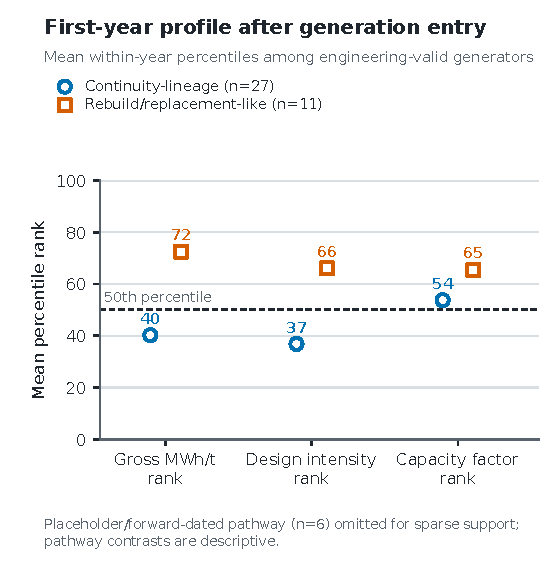
\includegraphics[width=0.72\textwidth,height=0.72\textheight,
  keepaspectratio]{figure4_post_entry_trajectories.pdf}
\caption[First-year profiles by reported entry pathway]{Mean within-fiscal-year percentile ranks in the first complete year
after reported entry for continuity-lineage entrants ($n=27$) and
rebuild/replacement-like entrants ($n=11$). Metrics are gross MWh/t, generator
design intensity (installed kW per t/day of processing capacity), and annual
electrical capacity factor among engineering-valid generator-years; the dashed
line marks the 50th percentile. The forward-dated/placeholder category
($n=6$) is omitted because support is sparse. All contrasts are descriptive.}
\label{fig:pathways}
\end{figure}

The larger descriptive pathway difference aligns more closely with generator
sizing than with capacity factor. This is not an estimated pathway effect:
assignment relies on reported resets, follow-up is selective, and there is no
counterfactual comparison between otherwise equivalent projects.

\section{Model coding and focal estimates}

\subsection{Technical formulas moved from the main narrative}

This appendix preserves the formal definitions used in the analysis while the
main methodology emphasizes the research logic and interpretation.

For installed-capacity and positive-output participation,
\begin{align*}
P_t^{K,\mathrm{all}}&=\frac{\sum_i I_{it}^{K}}{N_t}, &
P_t^{K,\mathrm{active}}&=\frac{\sum_i I_{it}^{K}I_{it}^{W}}{\sum_i I_{it}^{W}},\\
P_t^{G,\mathrm{all}}&=\frac{\sum_i I_{it}^{G}}{N_t}, &
P_t^{G,\mathrm{active}}&=\frac{\sum_i I_{it}^{G}}{\sum_i I_{it}^{W}}.
\end{align*}
Throughput and design-capacity coverage are
\[
P_t^{\mathrm{throughput}}=\frac{\sum_i W_{it}I_{it}^{G}}{\sum_i W_{it}},
\qquad
P_t^{\mathrm{design}}=\frac{\sum_i C_{it}I_{it}^{K}}{\sum_i C_{it}}.
\]
The valid-generator fleet identity is
\[
\frac{\sum_i G_{it}^{\mathrm{valid}}}{\sum_i W_{it}}
=\left(\frac{\sum_i W_{it}^{\mathrm{valid}}}{\sum_i W_{it}}\right)
\left(\frac{\sum_i G_{it}^{\mathrm{valid}}}{\sum_i W_{it}^{\mathrm{valid}}}\right).
\]
Firth estimation maximizes
\[
\ell_F(\boldsymbol{\theta})=\ell(\boldsymbol{\theta})+
\frac{1}{2}\log\left|\mathcal{I}(\boldsymbol{\theta})\right|.
\]
The predefined processing-scale contrast and standardized annual risk are
\[
OR_{300:100}=\exp(\beta_C\log 2),\qquad
\bar p(c)=\frac{1}{n}\sum_{i,t}
\operatorname{logit}^{-1}\!\left\{\mathbf{x}_{it}(c)'
\hat{\boldsymbol\theta}\right\}.
\]
The installed-capacity and capacity-factor models are
\begin{align*}
\log K_{it}&=\alpha_K+V_{it}'\beta_K+\beta_{KC}\log C_{it}
+T_{it}'\eta_K+\lambda_t+\varepsilon_{Kit},\\
\log F_{it}&=\alpha_F+V_{it}'\beta_F+\beta_{FC}\log C_{it}
+\beta_U U_{it}+T_{it}'\eta_F+\lambda_t+\varepsilon_{Fit}.
\end{align*}
With a common design matrix, the component regressions satisfy
\begin{align*}
\log D_{it}&=X_{it}'\gamma_D+e_{Dit}, &
\log F_{it}&=X_{it}'\gamma_F+e_{Fit},\\
\log U_{it}&=X_{it}'\gamma_U+e_{Uit}, &
\log Y_{it}&=X_{it}'\gamma_Y+e_{Yit},
\end{align*}
and therefore $\gamma_Y=\gamma_D+\gamma_F-\gamma_U$ for each cohort
contrast. This is an accounting identity, not a causal mediation result.

\subsection{First-entry model}

The first-entry likelihood includes only rows with $H_{it}=1$: at the start of
year $t$, lineage $i$ has no earlier observed positive installed-capacity
record. The four reported covariates are age per ten years,
$\log(1+C/100)$ for prior-year processing capacity $C$ in t/day, calendar time
per five years centred at FY2014.5, and $\log(1+R)$ for elapsed observed years
at risk. Table~\ref{tab:appendix-entry} reports every non-intercept coefficient
from the primary five-parameter Firth model and its three sensitivity frames.
Standard errors are fitted-model estimates; confidence intervals are
percentiles from 1,999 whole-lineage bootstrap replications.

The coefficient scale matters. The age estimate is a change in log odds for a
ten-year increase in prior reported age. Its broad-frame point estimate of
-0.327 corresponds to roughly 28\% lower odds, but the bootstrap interval
includes no association; it should not be converted into an age rule. The
processing-capacity coefficient applies to the transformed variable
$\log(1+C/100)$, not to a simple 100-tonne-per-day increment. The
300-versus-100 t/day odds ratio is therefore calculated as
$\exp(2.749\log 2)=6.72$. Standardized risks are easier to interpret because
they translate the same fit back to annual entries per 1,000 facility-years.

The two uncertainty summaries answer related but different questions.
Model-based standard errors describe the curvature of the fitted penalized
likelihood. The bootstrap intervals repeat the complete estimation after
resampling whole lineages, preserving within-lineage dependence and showing how
the estimate varies when the observed lineage composition changes. The thesis
uses the 1,999-lineage bootstrap for headline inference and retains model-based
quantities for transparent comparison and diagnostics.

Calendar time and elapsed observed risk remain in the model to prevent the
capacity coefficient from absorbing a simple panel-time pattern. They are not
interpreted separately because their strong correlation makes that separation
unstable. Technology and geography are omitted from the primary model because
35 events cannot support a large adjustment set; the leave-one-prefecture and
other sensitivity fits assess concentration but do not repair unmeasured
confounding.

\clearpage
\begingroup
\scriptsize
\setlength{\tabcolsep}{2.4pt}
\renewcommand{\arraystretch}{1.10}
\setlength{\LTleft}{\fill}
\setlength{\LTright}{\fill}
\begin{longtable}{L{2.95cm}L{2.75cm}R{1.25cm}R{1.35cm}L{2.35cm}R{0.9cm}}
\caption{Firth first-entry model focal coefficients}
\label{tab:appendix-entry}\\
\toprule
Frame & Term & Estimate & Model SE & Bootstrap 95\% CI & Events \\
\midrule
\endfirsthead
\toprule
Frame & Term & Estimate & Model SE & Bootstrap 95\% CI & Events \\
\midrule
\endhead
Broad exact-year (primary; 15,154 rows; 1,137 lineages) & Age per 10 years & -0.327 & 0.214 & -0.774 to 0.070 & 35 \\
Broad exact-year & Log processing capacity & 2.749 & 0.429 & 2.108 to 3.639 & 35 \\
Broad exact-year & Calendar time per 5 years & 0.696 & 0.277 & -0.012 to 1.149 & 35 \\
Broad exact-year & Log elapsed risk & -0.638 & 0.579 & -1.610 to 1.116 & 35 \\
Prior operation (13,072 rows; 1,019 lineages) & Age per 10 years & -0.323 & 0.231 & -0.793 to 0.147 & 33 \\
Prior operation & Log processing capacity & 2.825 & 0.487 & 2.030 to 3.783 & 33 \\
Prior operation & Calendar time per 5 years & 0.652 & 0.318 & -0.097 to 1.055 & 33 \\
Prior operation & Log elapsed risk & -0.497 & 0.643 & -1.469 to 1.347 & 33 \\
Same asset episode (15,095 rows; 1,135 lineages) & Age per 10 years & -0.751 & 0.271 & -1.364 to -0.206 & 24 \\
Same asset episode & Log processing capacity & 2.838 & 0.538 & 2.150 to 3.813 & 24 \\
Same asset episode & Calendar time per 5 years & 0.463 & 0.346 & -0.544 to 0.916 & 24 \\
Same asset episode & Log elapsed risk & 0.047 & 0.740 & -1.190 to 2.663 & 24 \\
Identity certain (15,107 rows; 1,130 lineages) & Age per 10 years & -0.328 & 0.214 & -0.791 to 0.065 & 35 \\
Identity certain & Log processing capacity & 2.758 & 0.429 & 2.081 to 3.620 & 35 \\
Identity certain & Calendar time per 5 years & 0.694 & 0.277 & -0.017 to 1.146 & 35 \\
Identity certain & Log elapsed risk & -0.639 & 0.580 & -1.552 to 1.067 & 35 \\
\bottomrule
\end{longtable}
\endgroup

The intercept is included in every fit but is not substantively interpreted.
Calendar time and elapsed risk are retained as nuisance controls and are not
interpreted separately because they are strongly correlated. Only the broad
exact-year frame is the primary model.

\clearpage
\subsection{Engineering outcome models}

The engineering models use 6,511 generator-years from 493 lineages and
lineage-clustered standard errors. Cohort contrasts use 2010 or later as the
reference. Shared controls are log processing capacity, furnace count, furnace
group, facility group, and fiscal-year indicators. The omitted categories are
fluidized-bed furnace, gasification/melting facility, and FY2005; these are
coding references rather than normative comparison standards. The
capacity-factor model additionally includes waste-processing utilization. The
gross-output model replaces log processing capacity with log annual throughput
and log installed capacity.

\begingroup
\scriptsize
\setlength{\tabcolsep}{2.4pt}
\renewcommand{\arraystretch}{1.10}
\setlength{\LTleft}{\fill}
\setlength{\LTright}{\fill}
\begin{longtable}{L{3.0cm}L{3.15cm}R{1.2cm}R{1.25cm}L{2.25cm}R{0.7cm}}
\caption{Engineering model focal coefficients}
\label{tab:appendix-engineering}\\
\toprule
Outcome & Term & Estimate & Clustered SE & 95\% CI & $R^2$ \\
\midrule
\endfirsthead
\toprule
Outcome & Term & Estimate & Clustered SE & 95\% CI & $R^2$ \\
\midrule
\endhead
Log installed capacity (kW) & Before 1990 cohort & -1.565 & 0.084 & -1.730 to -1.399 & 0.786 \\
Log installed capacity (kW) & 1990--1999 cohort & -0.883 & 0.063 & -1.007 to -0.758 & 0.786 \\
Log installed capacity (kW) & 2000--2009 cohort & -0.267 & 0.043 & -0.352 to -0.183 & 0.786 \\
Log installed capacity (kW) & Log processing capacity & 1.532 & 0.044 & 1.447 to 1.617 & 0.786 \\
Log capacity factor & Before 1990 cohort & 0.302 & 0.042 & 0.220 to 0.384 & 0.339 \\
Log capacity factor & 1990--1999 cohort & 0.198 & 0.032 & 0.135 to 0.262 & 0.339 \\
Log capacity factor & 2000--2009 cohort & 0.015 & 0.029 & -0.042 to 0.072 & 0.339 \\
Log capacity factor & Log processing capacity & -0.116 & 0.024 & -0.162 to -0.070 & 0.339 \\
Log capacity factor & Waste-processing utilization & 1.695 & 0.126 & 1.448 to 1.942 & 0.339 \\
Log gross generation (MWh) & Log annual throughput & 0.638 & 0.052 & 0.536 to 0.740 & 0.914 \\
Log gross generation (MWh) & Log installed capacity & 0.576 & 0.038 & 0.502 to 0.650 & 0.914 \\
\bottomrule
\end{longtable}
\endgroup

Table~\ref{tab:appendix-engineering} reports every focal coefficient used for
the RQ3 interpretation. Furnace-group, facility-group, furnace-count,
fiscal-year, and intercept coefficients are nuisance adjustments rather than
thesis estimands. Sections 3.5.1--3.5.3 define the models and variables; Tables
4--5 and Appendix Tables B1--B2 report the estimates needed to evaluate the
three principal research questions within this document.

\end{document}
